\documentclass[12pt]{extarticle}
\usepackage[english]{babel}
\usepackage{NotesTeX}
\usepackage{subfigure}
\usepackage{tikz}
\usetikzlibrary{arrows}
\usepackage{multirow}
\usepackage{listings}
\usepackage{extarrows}
\usepackage{parskip}
\usepackage{eurosym}
\usepackage{footmisc}

\graphicspath{{../output/}}
\collaborationImg{
\includegraphics[width=30mm]{../../pictures/UIO.png}}

\author{\Large Håkon Olav Torvik, Vetle Vikenes \& Sigurd Sørlie Rustad}
\title{\Huge Machine Learning: Using regression and neural networks to fit continuous functions and classify data}
\affiliation{\large FYS-STK4155 – Applied Data Analysis and Machine Learning
\\Autumn 2021\\Department of Physics\\University of Oslo\\\\\today}
\begin{document}
\abstract{
	Abstract coming soon.
}
\maketitle
\pagestyle{myplain}

% TODO!!

% Rapport:

% !! ABSTRACT !!

% SGD: Franke
%  - Bestemme beste parametere
%  - Regne ut mse for de
%  - Få metode til å stemme med resultater

% NN: Franke
%  - Regne den beste MSE-verdien
%  - Få metode til å stemme med resultater

%  - Sammenligne SGD og NN med OLS

% NN: Cancer
% alt. Metode og resultat
% (figurene er laget)
% Implementere strengere klassifikasjon
% Plotte cost

% Logreg: Cancer
% DONE

% Annet:
% Diskusjon
% Andre, uavhengige analyser vi har gjort? (simple.py, MNIST)

% Kode:
% README for code directory, hvis ikke: opdater readme i project2 mappa.
% Rydde code

\section{Introduction}
In the modern world, digital data has become one of the most valuable commodities there is. Not because of scarcity, like most other valuables, but rather the exact opposite; the vast abundance of data available makes being able to understand trends and patterns in it extremely valuable for companies looking for profit. However, data is complex, having many features, and understanding how one affect another can be impossible with human analysis alone. Luckily, there exists statistical methods that let us find the deeper connections, make models and even predict outcomes. In this paper we wish to study some stochastic methods, and look at their limitations and strengths.

First we will study a bi-variate continuous function known as the Franke function. We will use both stochastic gradient descent and a feed-forward deep neural network, with back propagation. Then we can also compare results with those obtained in a previous paper, using the deterministic methods ordinary least squares and ridge regression. Note that all methods used in this report is briefly covered in the theory section.

Next we will embark on a classification problem, using measurments of tumors in breast tissue to predict wether they are benign or malignant. Here we will again use a feed-forward deep neural network, along with logistic regression.

We will in no way answer all questions linked to the aforementioned methods. So that anyone can reproduce or continue our studies, we list all the code, results and instructions on running the code in our GitHub repository\footnote{\href{https://github.com/sigurdru/FYS-STK4155/tree/main/project1}{https://github.com/sigurdru/FYS-STK4155/tree/main/project2}}.

\section{Theory}
In the theory-section we aim to give a brief explanation of the main concepts and terminology used in this report. For a more in-depth explanation we recommend reading the appropriate sections in \cite{2019}, which has been of great inspiration and help for us throughout the project.

In general, we have a dataset $\bo x$, where each point $\bo x_i$ takes a value $y_i$, for which we want to make a model $\bbeta$, such that for a new data point $\bo x_k \notin \bo x$ we can make a prediction for the value $y_k$.  The model $\bbeta$ is a vector/matrix, where each element is a parameter of our model, such that $\bbeta$ is sometimes called the parameters. For gradient descent, we have to choose what shape the model should be, as was done for linear regression in \cite{project1}, while the neural network makes its own model.

\subsection{Gradient Descent}\label{sec:GD}
In this section we cover gradient descent and different variations of it. More specifically we describe gradient descent (GD), stochastic gradient descent (SGD) and adding momentum to the aforementioned methods. All gradient descent methods start with an initial guess for what the model $\bbeta$ should be, and iteratively updates the guess by training on the dataset, either until it reaches a minimum, or a certain number of iterations have been performed.
\subsubsection{Ordinary Gradient Descent}
Gradient descent methods is often used to minimize the so-called cost/loss-function, which tells us how good our model at predicting the dataset is (more on this in section \ref{sec:cost_func_and_regul}). For now, we use a general cost function $C(\bbeta)$ for a given model $\bbeta$, which can be expressed as the sum over the cost function for each datapoint $\bo x_i$, as such:
\begin{equation}
	C(\boldsymbol{\beta}) = \sum_{i = 1}^{n}c_i(\mathbf{x}_i, \boldsymbol{\beta}),
\end{equation}
where $n$ denotes the number of datapoints. The gradient with respect to the parameters $\bbeta$, which represent the direction of optimal minimization of the cost function,  is then defined as
\begin{align}
	\nabla_{\boldsymbol{\beta}} C(\boldsymbol{\beta}) = \sum_{i = 1}^{n} \nabla_{\boldsymbol{\beta}} c(\mathbf{x}_i, \boldsymbol{\beta}).
	\label{eq:Total_gradient}
\end{align}
The algorithm for GD is then:
\begin{align}
	\mathbf{v}_t             & = \eta \nabla_{\boldsymbol{\beta}} C(\boldsymbol{\beta}_t) \nonumber \\
	\boldsymbol{\beta}_{t+1} & = \boldsymbol{\beta}_t - \mathbf{v}_t,
	\label{eq:GD_algo}
\end{align}
where $\eta$ is what we call the learning rate, representing the step-length to move in the optimal direction.  This algorithms iteratively finds a new $\boldsymbol{\beta}_{t+1}$ which (ideally) decreases the cost function. This is of course not always the case, and depends on the value of $\eta$.

For a model with $p$ parameters, the cost-function is the surface of a $p$-dimensional hypersurface, and minimizing this can lead to several problems. For example, if $\eta$  is too big, the cost-function can diverge and never find a minimum of the hypersurface, while if $\eta$ is too small we will need too many iterations to reach a minimum in reasonable time. One method of avoiding the cost-function diverging, is using a dynamic learning schedule, where the learning rate $\eta$ decreases during training. The model then makes larger steps in the beginning, and then smaller and smaller, such that we should be able to converge to a minimum, and not making too big steps, circling around it.

An additional problem is that the  hypersurface is not a smooth terrain with a single minimum. Our model can potentially move down into a local minimum, which can be close to the level of the global minimum, or far worse than it. When our model converges, we have no way of knowing if we have found the optimal, global minium, or are stuck in one of the many local minima, with no way of getting out.


\subsubsection{Stochastic Gradient Descent}\label{sec:SGD}
With large datasets, a large number of computations is needed when calculating the gradient. It takes a lot of time, and the model is only updated once per iteration, making improvement slow. Stochastic Gradient Descent. SGD, combats this by approximating the total gradient \eqref{eq:Total_gradient}. This is done by performing  gradient descent on a subset of the data, called a minibatch. With $n$ still denoting the total number of datapoints, we will have $N_B=n/M$ minibatches, where $M$ is the size of each minibatch. The minibatches are denoted by $B_k$. Thus our approximated gradient for a single minibatch $B_k$ is defined as
\begin{align}
	\nabla_{\boldsymbol{\beta}} C^{MB}(\boldsymbol{\beta}) \equiv \sum_{i \in B_k}^M \nabla_{\boldsymbol{\beta}} c(\mathbf{x}_i, \boldsymbol{\beta}).
\end{align}
Then the aim is to use this approximated gradient, for all $N_B$ minibatches, to update the parameters $\boldsymbol{\beta}$, at every step $k$. Doing this for all $N_B$ minibatches, are what we refer to as an epoch. The SGD algorithm then becomes very similar to \eqref{eq:GD_algo}, however with an approximated gradient.
\begin{align}
	\mathbf{v}_t             & = \eta\nabla_{\boldsymbol{\beta}} C^{MB}(\boldsymbol{\beta}_t) \nonumber \\
	\boldsymbol{\beta}_{t+1} & = \boldsymbol{\beta}_t - \mathbf{v}_t
	\label{eq:SGD_algo}
\end{align}
Choosing a smaller $M$ gives a worse approximation of the full gradient, though at the same time the model will have more chances to move in the correct direction. Further, by choosing $M$ such that $N_B$ is neither too small or large, our program will run faster. This not only speeds up our program, it also helps prevent getting stuck in local minima because of the stochastic nature. The dataset is shuffled after each epoch, creating new minibatches such that we never use the same one twice.

\subsubsection{Adding Momentum}
These methods can still be optimized further by adding momentum. This is done by adding a term to the parameter $\mathbf{v}_t$ in equations \eqref{eq:GD_algo} and \eqref{eq:SGD_algo}. This so-called mass term, simulates the gradient having momentum, such that every update of $\bbeta$ is a running average.
\begin{align} \label{eq:vt_mom}
	\mathbf{v}_t = \eta \nabla_{\boldsymbol{\beta}_t} C(\boldsymbol{\beta}) \rightarrow \mathbf{v}_t = \gamma \mathbf{v}_{t-1} + \eta \nabla_{\boldsymbol{\beta}} C(\boldsymbol{\beta}_t).
\end{align}
Here $\gamma \in [0, 1]$ is what we could refer to as the mass, and is a free parameter. One of the benefits is for example that this lets us move faster in regions where the gradient is small.

\subsection{Logistic Regression}\label{sec:logistic_regression}
Logistic Regression is used for classification problems, meaning that we want to predict discrete outputs, for instance true or false, given a set of information about a subject. This is the case for binary classification, where we only have one output. It is also possible to use multi-class classification, where one has several outputs, each representing the probability of the class being given by that output. In our case we want a model that takes in some values $\mathbf{x}_i$ and spits out zero or one. These values should correlate with the actual classification $y_i\in\{0,1\}$ corresponding to true or false respectively. Lets define our model as
\begin{align}
	\sigma(s_i), \ \ \text{where }s_i = \bo x_i^T \bo w + b_0 \equiv \bo X_i^T \bo W,
	\label{eq:log_reg_model}
\end{align}
where $\bo x_i^T$ is our inputdata, $\bo w$ and $b_0$ are parameters in the model. As a shorthand we also defined $\bo W = (b_0, \bo w)$ and $\bo X_i = (1, \bo x_i)$. We also have $\sigma$ which is some soft classifier that maps our output between zero and one (i.e. the sigmoid \eqref{eq:sigmoid}). The reason why we want a soft classifier and not a hard one (like $\sigma = 1$ if $s\geq0$ and $0$ otherwise), is because then we can interpret the output as a probability, quantifying how certain the model is in its prediction. Here we also need a cost function to minimize. It is common to choose the cross entropy, which we derive in \ref{sec:cost_func_and_regul}. However we will just use it without derivation for now. The cross entropy for this model is given as
\begin{align}
	C(\bo W) = \sum_{i = 1}^{n} -y_i \log\sigma(\bo X_i^T \bo W) - (1 - y_i)\log\left[1 - \sigma(\bo X^T_i \bo W)\right],
	\label{eq:cross_entropy2}
\end{align}
where $n$ are the number of samples we want to classify, and $y_i$ the true classification. Now with a cost function and model in hand we are ready to minimize the cost function in order to find the optimal parameters for the model. The gradient of the cost function is given by
\begin{align}
	\nabla_{\bo W} C(\bo W) = \sum_{i = 1}^n \left[\sigma(\bo X_i^T \bo W - y_i)\right]\bo X_i.
	\label{eq:cross_entropy_grad}
\end{align}
Thus the only thing left to do is perform an algorithm similar to \ref{eq:SGD_algo}, where the parameters to update are $\bo W$.

\subsection{Feed-Forward Deep Neural Networks}\label{sec:NeuralNetwork}
Neural networks are neural-inspired nonlinear models, which are taught by a way of learning. We will in this section explain what we mean by non-linearity, the basic architecture of a neural network and how the network \emph{learns}. In this paper, only supervised learning will be studied, where we train our model on fully labeled data, as opposed to unsupervised learning, where the model first is shown unlabeled data.

\subsubsection{Architecture of Neural Networks}
%The structure we are going to use in this report is similar to that in figure \ref{fig:neural_network}. The gray circles are what we refer to as nodes. For now we just need to know that they hold some numerical value. One initializes the network by giving the nodes in the input layer numerical values. These values would correspond to some actual physical property, for example brightness of pixels in a picture. Then, each node in the input layer is connected to each node in the hidden layer $h_1$. In figure \ref{fig:neural_network} we have three such hidden layers, where each node in one layer is connected to every node in the next layer. Now the nodes are connected through what we will refer to as weights, biases and activation functions (more on that later). The connections are what assigns the numerical value of the nodes in the next layer. Lastly we have the output layer, which outputs values dependent on the problem. If we have a classification situation, where we for example wanted to classify the type of animal in different pictures, then one node could correspond to  a lion, next to a zebra and so fourth. By this we would know what animal the network \emph{thinks} is in the picture by looking at what neuron has the highest numerical value.

The structure of the neural net we will use in this report is similar to that in figure \ref{fig:neural_network}. The gray circles are what we refer to as nodes, and are organized into layers. They hold some numerical value. The first and last layer are the input and output layer, respectively. The rest are so-called hidden layers, denoted $h_i$. In figure \ref{fig:neural_network} there are three hidden layers. Between each layer is a set of weights, connecting each node in the preceding layer to each node in the succeeding one. One initializes the network by giving the nodes in the input layer numerical values. These values would correspond to some actual physical property, for example brightness of pixels in a picture. Then, the values are fed forward, where the values of the nodes in the next layer being the weighted sum of the values in the previous, plus a bias $b$. The values are \textit{activated} by an activation function, before similarly being fed forward to the next layer, until reaching the output layer. In the case of regression, the output layer is a single node, giving the functional value. In the case of classification, for example classifying the type of animal in pictures, one node could correspond to a lion, next to a zebra and so fourth. By this we would know what animal the network predicts is pictured by finding the neuron has the highest numerical value.

\begin{figure}[h]
	\minipage{0.70\textwidth}
	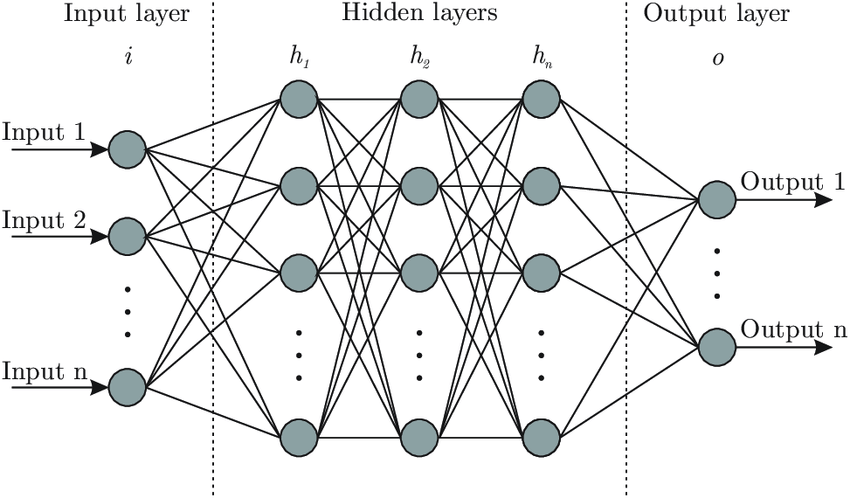
\includegraphics[width=\linewidth]{pictures/neural_network.png}
	(source: \texttt{https://www.researchgate.net/figure/Artificial-neur
		al-network-architecture-ANN-i-h-1-h-2-h-n-o\_fig1\_321259051})
	\endminipage\hfill
	\minipage{0.29\textwidth}
	\caption{Basic outline of a neural network. It displays the different layers (input, hidden and output), nodes (gray circles) and the connection between the nodes (black lines).}\label{fig:neural_network}
	\endminipage
\end{figure}

We mentioned that the different nodes are connected through weights, biases and activation functions. Looking at figure \ref{fig:neural_network}, a neuron $j$ in layer $h_1$ is connected to $n$ input neurons, denoted by black lines. Each input neuron has a numerical value defined by the problem. The value neuron $j$ in $h_1$ then gets is defined as
\begin{align}
	a_{h_1, j} = \sigma (x_1w_1 + x_2w_2 + \dots + x_nw_n + b_j),
\end{align}
where $x_i$ are the values of neuron $i$ in the input layer, $w_i$ are the weights between neurons $i$ and $j$, $b$ is what we refer to as the bias and $\sigma$ is the activation function. Every neuron is connected like this, with different weights and biases. Initially the network will make random predictions. Through training, the weights and biases are updated using the backpropagation algorithm, described in section \ref{sec:back_prop}.

\subsubsection{Activation Functions}\label{sec:teo:act_funcs}
The activation functions are where the non-linearity of the neural nets comes in, because they are non-linear. Now there are many such functions, in our project we have implemented the 3 displayed in figure \ref{fig:activation_functions}. The exact functions are as follows
\begin{align}
	\text{Sigmoid: }\sigma(x)    & = \frac{1}{1 + e^{-x}},\label{eq:sigmoid}          \\
	\text{RELU: }\sigma(x)       & = \max(0,x), \label{eq:RELU}                       \\
	\text{Leaky RELU: }\sigma(x) & = \begin{cases}
		\alpha x, & \text{if } x\leq 0 \\
		x,        & \text{otherwise}.
	\end{cases} \label{eq:leaky_RELU}
\end{align}
For Leaky RELU, $\alpha$ is some parameter which we set to $\alpha = 0.01$. As we will show in section \ref{sec:back_prop}, the derivative of the activation function is used to update the weights and biases of the network. It can happen that inputs to the activation function of nodes are negative, making the derivative of the RELU function zero, such that the contribution from these neurons to the learning of the network vanishes. This is the main benefit of using Leaky RELU, as this won't happen. However, using good weight initialization, this should not be a problem, so we do not expect the difference between the two activation functions to be very significant.

\begin{figure}[h]
	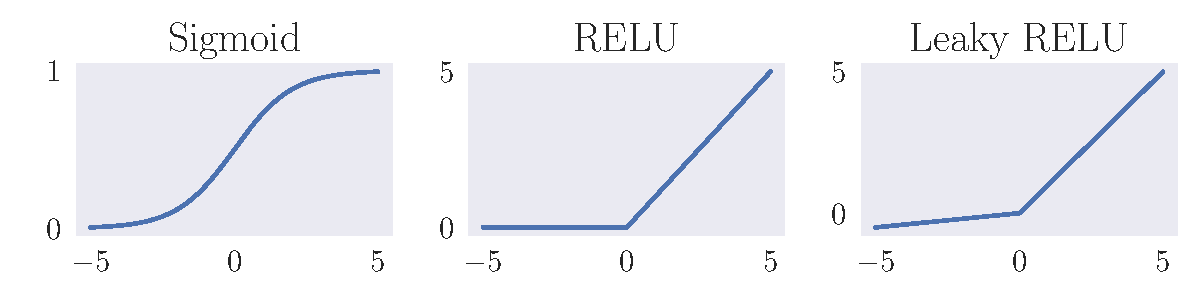
\includegraphics[width=\linewidth]{pictures/activation_functions.pdf}
	\caption{Some activation functions, sigmoid, RELU and Leaky RELU, respectively.}\label{fig:activation_functions}
\end{figure}

All neurons in all hidden layers are activated by the same activation function. The input layer is just the input, so it is not activated. In the case of regression, the output layer is not activated. Then the predicted function value is just the weighted sum from the last hidden layer. For classification, we want the values in the output nodes to indicate probabilities. Thus, we use an activation function that considers the value in the other nodes in the other output nodes. The softmax function does this

\begin{equation} \label{eq:softmax}
	\sigma(z_i) = \frac{e^{z_i}}{\sum_{j=1}^Ke^{z_j}},
\end{equation}
where $K$ is the number of classes, output nodes.

\subsubsection{Cost Function and Regularization}\label{sec:cost_func_and_regul}
Before one can start training the data, we must have a cost function. This will quantify how well or poorly our network is performing, and is what we want to minimize when we train the network. For continuous data it is common to use mean square error (MSE) as the cost function. It is just the difference between desired output ($\hat{\mathbf{x}}$) and actual output ($\mathbf{x}$), squared, averaged over all datapoints $\bo x_i$, as such
\begin{align}
	C(\mathbf{x}) = \frac{1}{n}\sum_{i=1}^{n}(\hat{\mathbf{x}}_i - \mathbf{x}_i)^2.
	\label{eq:MSE}
\end{align}

As was done with linear regression, \cite{project1} regularization can help prevent overfitting. Common regularization methods are $L_1$ and $L_2$ penalties, which add a regularization term to the cost function, as such
\begin{align}
	L_1: \ \ C(\mathbf{x}) & = \frac{1}{n}\sum_{i=1}^{n}(\hat{\mathbf{x}}_i - \mathbf{x}_i)^2 + \lambda\sum_j \abs{\mathbf{W}_j}, \label{eq:L1} \\
	L_2: \ \ C(\mathbf{x}) & = \frac{1}{n}\sum_{i=1}^{n}(\hat{\mathbf{x}}_i - \mathbf{x}_i)^2 + \lambda\sum_j \mathbf{W}^2_j, \label{eq:L2}
\end{align}
where $\lambda$ is some regularization parameter and $\mathbf{W}$ are the weights and biases. We will in this paper study the effects of adding a $L_2$-regulizer term when updating the parameters, by adding the term $\eta \lambda \mathbf{W}_{t-1}$ to equation \eqref{eq:vt_mom}.

We mentioned when talking about logistic regression (section \ref{sec:logistic_regression}), that for classification scenarios one will often use cross-entropy as the cost function. Continuing with the model defined by \eqref{eq:log_reg_model}, we want to find an appropriate cost function. We define the probability of an outcome $y_i$ given parameters $\bo X_i$ and $\bo W$ as
\begin{align}
	P(y_i = 1|\bo X_i, \bo W) & = \frac{1}{1 + \exp(-\bo X_i^T \bo W)}, \\
	P(y_i = 0|\bo X_i, \bo W) & = 1 - P(y_i = 1|\bo X_i, \bo W)
\end{align}
We can then map these probabilities to our soft classifier $\sigma(s_i)$
\begin{align}
	P(y_i = 1) = \sigma(s_i) = \sigma(\bo X_i^T \bo W).
\end{align}
Now we can define the cost function using Maximum Likelihood Estimation (MLE), which states that we should choose parameters that maximize the probability of our given data. Consider the dataset $\mathcal{D}\{(y_i, \bo x_i)\}$, where we remind that $\bo x_i$ are the input parameters. Then the probability of our dataset given $\bo W$ is
\begin{align}
	P(\mathcal{D}|\bo W) = \prod_{i=1}^{n} \left[\sigma(\bo X_i^T\bo W)\right]^{y_i} \left[1 - \sigma(\bo X_i^T\bo W)\right]^{(1 - y_i)}.
\end{align}
Again we remind that $n$ are the number datapoints we want to classify. This expression is difficult to work with, thus we take the logarithm.
\begin{align}
	l(\bo W) = \log(P(\mathcal{D}|\bo W)) = \sum_{i = 1}^n y_i\log(\sigma(\bo X_i^T \bo W)) + (1-y_i)\log(1 - \sigma(\bo X_i^T \bo W))
\end{align}
MLE entails finding the $\bo W$ that maximizes $l(\bo W)$, or more commonly, minimizes $-l(\bo W)$. Thus our cost function becomes
\begin{align}
	C(\bo W) = -l(\bo W) = \sum_{i = 1}^{n} -y_i \log\sigma(\bo X_i^T \bo W) - (1 - y_i)\log\left[1 - \sigma(\bo X^T_i \bo W)\right],
	\label{eq:cross_entropy}
\end{align}
which is equation \eqref{eq:cross_entropy2}.

\subsubsection{The Backpropagation Algorithm} \label{sec:back_prop}
With a desired cost function we are ready to train the neural network. This is done by the backpropagation algorithm. The method entails finding the derivative of the cost function, with respect to all parameters. When we have a neural network, we have thousands of parameters which can be tuned (weights and biases), meaning that we have to approximate the derivative somehow. The backpropagation algorithm does just that, by exploiting the layered structure displayed in figure \ref{fig:neural_network}.

Before we can embark on deriving the algorithm we will introduce some notation. We assume $L$ total layers, indexed as $l = 1, \dots , L$. Next we need to index the weights, nodes and biases. Let $w_{jk}^l$ be the weight connecting $k$-th neuron in layer $l-1$ and $j$-th neuron in layer $l$. The index order in $j$ and $k$ are such that we can do matrix multiplication with index notation later down the road. Further let $b_j^l$ be the bias for the $j$-th neuron in layer $l$. Thus the activation of the $j$-th neuron in layer $l$ ($a^l_j$) becomes
\begin{align}
	a_j^l = \sigma\left(\sum_{k} w_{jk}^l a_k^{l-1} + b_j^l\right) = \sigma(z_j^l), \ \ z_j^l \equiv \sum_{k} w_{jk}^l a_k^{l-1} + b_j^l.
	\label{eq:activation_of_node_ajl}
\end{align}
Here $\sigma$ is an activation function.

Now the cost function will depend directly on the activation of the output layer ($a^L_j$). However the activation of the output layer depends on the previous layers, meaning that the cost function depends indirectly on all the previous layers. Lets define define the error $\Delta_j^L$ of the $j$-th neuron in layer $L$, as the change in cost function with respect to $z^L_j$.
\begin{align}
	\Delta_j^L \equiv \del{C}{z_j^L}
	\label{eq:backprop0}
\end{align}
We can similarly define the error of neuron $j$ in layer $l$, as the change in the cost function with respect to $z_j^l$,
\begin{align}
	\Delta_j^l \equiv \del{C}{z_j^l} = \del{C}{a_j^l}\del{a_j^l}{z^l_j} = \del{C}{a_j^l}\der{\sigma(z^l_j)}{z^l_j}.
	\label{eq:backprop1}
\end{align}
In the next few lines we are going to derive several equations needed for the algorithm, it will be apparent why after we have found them. Notice that \eqref{eq:backprop1} also can be written as
\begin{align}
	\Delta_j^l = \del{C}{z_j^l} = \del{C}{b_j^l}\del{b_j^l}{z^l_j} = \del{C}{b_j^l}.
	\label{eq:backprop2}
\end{align}
Because $\partial b_j^l/\partial z^l_j = 1$ from \eqref{eq:activation_of_node_ajl}. Again using the chain rule we can rewrite \eqref{eq:backprop1}
\begin{align}
	\Delta_j^l & = \del{C}{z_j^l} = \sum_{k} \del{C}{z_k^{l+1}}\del{z_k^{l+1}}{z^l_j} = \sum_{k} \Delta_k^{l+1}\del{z_k^{l+1}}{z^l_j} \nonumber \\
	           & = \left(\sum_{k} \Delta_k^{l+1} w_{kj}^{l+1}\right)\der{\sigma(z^l_j)}{z^l_j}.
	\label{eq:backprop3}
\end{align}
To find the last equation, we differentiate the cost function with respect to the weight $w^l_{jk}$
\begin{align}
	\del{C}{w_{jk}^l} = \del{C}{z_j^l}\del{z_j^l}{w_{jk}^j} = \Delta l a_k^{l-1}.
	\label{eq:backprop4}
\end{align}
The equations \eqref{eq:backprop1}, \eqref{eq:backprop2}, \eqref{eq:backprop3} and \eqref{eq:backprop4} define what we call the backpropagation algorithm. Then, what exactly is the algorithm? It entails six steps:
\begin{description}
	\item[1 Activation:] First activate the neurons in the activation layer ($a^1_j$) with desired data.
	\item[2 Feedforward:] Activate the nodes in following layers, this is done by equation \eqref{eq:activation_of_node_ajl}.
	\item[3 Error at layer $L$:] Calculate the error at the last layer using \eqref{eq:backprop1}.
	\item[4 Backpropagate error:] With \eqref{eq:backprop3} we can the calculate the error, iterating backwards in the network.
	\item[5 Calculate gradient:] Find the gradient by using equations \eqref{eq:backprop2} and \eqref{eq:backprop4}.
	\item[6 Update parameters:] Update the parameters similarly to \eqref{eq:SGD_algo}, however $\boldsymbol{\beta}_t$ are our weights and biases in this case.
\end{description}

The expression for updating the weights and biases are
\begin{align}
	w_{jk}^l \leftarrow & w_{jk}^l - \eta \Delta_j^l a_k^{l-1} \label{eq:update_weights} \\
	b_j^l \leftarrow    & b_j^l - \eta \Delta_j^l \label{eq:update_biases}
\end{align}

\subsubsection{Numerical gradients} \label{sec:num_gradients}
When computing the derivatives involved in the backpropagation algorithm numerically, we will mainly use the autograd module in python. The exception to this is when we deal with classification and use the cross-entropy cost function (equation \eqref{eq:cross_entropy}) combined with the softmax activation function (equation \eqref{eq:softmax}) for the output layer. It can be shown analytically, that the error, equation \eqref{eq:backprop1}, of the output layer in this case can be written as
\begin{align} \label{eq:softmax_crossentropy_derivative}
	\Delta_j^L & = \del{C}{a_j^L}\der{\sigma(z_j^L)}{z_j^L} = a_j^L - y_j
\end{align}
where $a_j^L$ is the $j$-th node of the output layer, and $y_j$ is the corresponding target value.

\subsubsection{Initialization of weights} \label{sec:wi}
We mentioned earlier that the network has weights and biases between the layers. These needs to be initialized in some way. The biases are simple to initialize, as they are a single number for every node. These are initialized as a small, non-zero value $b_0$.

Before 2006, most neural networks were performing quite badly on most tasks, as they did not learn during training. One of the (several) reasons were due to bad initialization of weights. A common way of doing this was using the standard normal distribution $W_{i,j} \sim  \mathcal{N}(0, 1)$. The problem with this is that it does not consider the size of the layers. In 2010, it was shown that when using sigmoid as the activation function, Xavier-initialization give better results \cite{xavier}. This is given as $W_{i, j}\sim\mathcal{U} \left(-\frac{1}{\sqrt{n}}, \frac{1}{\sqrt{n}} \right)$, where $\mathcal{U}$ is the uniform distribution, and $n$ is the number of nodes in the preceding layer.

In 2015, He-initialization was shown to work well with ReLU and Leaky ReLU \cite{He}. Here, the weights are initialized using the normal distribution, but with a variance given by $v = 2/(1 + \alpha^2)n$, where again $n$ is the number of nodes in the preceding layer, and $\alpha$ is the parameter of the Leaky ReLU-function. For ReLU, this is 0. This initialization only considers the number of nodes in the preceding layer, though normalized initialization where the number of nodes in the succeeding layer is considered as well could yield better results. We use the forementioned method to initialize the network for the appropriate activation-function, and will not study other methods of initialization.



\section{Methods}
As we mentioned in the introduction, we wish to study different ways of fitting two types of datasets. The first is fitting the \textit{continuous} Franke Function \eqref{eq:FF}, i.e. regression. We will use both stochastic gradient descent and feed forward neural network to fit the data. Both methods are covered in the theory sections \ref{sec:GD} and \ref{sec:NeuralNetwork} respectively.

Next we will embark on an classification problem. Namely predicting if breast tumors are malignant or benign, using the Breast Cancer Wisconsin data set\footnote{\href{https://www.kaggle.com/uciml/breast-cancer-wisconsin-data}{https://www.kaggle.com/uciml/breast-cancer-wisconsin-data}}. We will again use our feed forward neural network, as well as logistic regression. The latter is covered in the theory section \ref{sec:logistic_regression}.

\subsection{Franke Function}
\begin{align}
	\begin{split}\label{eq:FF}
		f(x,y) = &\frac{3}{4}\exp(-\frac{(9x -2)^2}{4} - \frac{(9y-2)^2}{4}) + \frac{3}{4}\exp(-\frac{(9x + 1)^2}{49} - \frac{(9y + 1)}{10})
		\\
		+ &\frac{1}{2}\exp(-\frac{(9x-7)^2}{4} - \frac{(9y -3)}{4}) - \frac{1}{5}\exp(-(9x-4)^2 - (9y-7)^2).
	\end{split}
\end{align}
In \cite{project1}, we already studied the Franke function using linear regression, specifically OLS and OLS with an L2 and L1 parameter $\lambda$, so-called Ridge and Lasso regression. The results from these methods will form the basis for comparing our results using SGD and neural networks. The report, along with the code can be found at our GitHub\footnote{\href{https://github.com/sigurdru/FYS-STK4155/tree/main/project1}{https://github.com/sigurdru/FYS-STK4155/tree/main/project1}}. In order to have comparable results, we will use the same parameters for the data. Only the methods will be different. In that project we generated the data using $N=30\times30$ uniformly distributed datapoints in $x$- and $y$-direction, respectively. To simulate it being real data, we also added normally distributed noise with mean zero and standard deviation $0.2$: $\epsilon \sim \mathcal{N}(0,0.2)$. We also split the input and target data in the same way as before, using $80\,\%$ of the data for training and $20\,\%$ of the data for testing. The two splitted data sets are then scaled by subtracting the mean of the relevant training data.

\subsubsection{Stochastic Gradient Descent}
As in \cite{project1}, we have to choose a model to fit the data to, when using SGD. The simplest is a bi-variate polynomial of degree $P$, such that our model will have $p$ features. This is the design matrix $X$ used in the previous project. Having obtained good results for OLS using $P = 6$, we use the same polynomial degree for SGD. Writing our own code for implementing SGD, we will analyze the results with MSE (equation \eqref{eq:MSE}) as our cost function for various parameters. We include the $L_2$ regularization term, equation \eqref{eq:L2}, in the gradient of the cost function, which gives the gradient corresponding to Ridge regression. The expression for the stochastic gradient is given in equation \eqref{eq:SGD_gradient}

\begin{align} \label{eq:SGD_gradient}
	\nabla_{\boldsymbol{\beta}}C^\mathrm{MB} (\boldsymbol{\beta})=2 X^T (X \boldsymbol{\beta} - \boldsymbol{z})/M + 2\lambda\boldsymbol{\beta}
\end{align}

where OLS regression is obtained by setting $\lambda=0$. There are multiple parameters to consider for stochastic gradient descent, and the ones we will study are the choice of learning rate $\eta$, number of epochs $N_e$, number of minibatches $N_B$, regularization parameter $\lambda$, and the momentum parameter $\gamma$. This gives us a 5-dimensional hyper-parameter space, and we would ideally optimize each parameter to get the lowest possible MSE. This could be done by grid search, where we test a range of values for every parameter. Testing, for instance, 10 values of each parameter at once means that we have to run the algorithm $10^5$ times, which makes the process extremely slow. We will therefore simplify our search, only doing grid search over 1 or 2 of the parameters at a time, keeping the rest constant. We then study how each parameter affects the results, independently of the other parameters.

%TROR IKKE VI BURDE SI DETTE:
%Further, it is not too valuable to find the absolutely optimal parameters in our hyperparameter space, because there are many more parameters we will not controll for, like the noise in the data or polynomial degree of our model.

We begin by studying the MSE of the Franke function. For the MSE values we will include the result from both the train and test data in our first simulation only, confirming that overfitting eventually takes place, while focusing on the test MSE in all the remaining simulation, which is the result of interest. The MSE is studied for different values of $\eta$ as a function of $N_e\in[0,\,150]$, setting $\lambda=\gamma=0$ and $N_B=20$, i.e. minibatches of size $M=36$ for the $720$ points in the training dataset. We choose $21$ evenly spaced values of $\eta\in[0.01,\,0.9]$.

We then choose one of the favorable learning rates to study the MSE for minibatch sizes of $M\in[720,\,360,\,240,\,144,\,72,\,48,\,36,\,30,\,24]$, as a function of epochs, using $N_e\in[0,\,150]$ once again. The values of $M$ are chosen such that $N_B$ becomes integers. This does not have to be the case, but will make the results more consistent. Next, using $N_B=20$ minibatches, we then study the MSE after $N_e=150$ epochs as a function of $\eta$ and $\lambda$ to study the effect of regularization. For this we use $11$ linearly distributed values of $\eta\in[0.1,\,0.5]$ and $11$ uniformly distributed values of $\lambda\in[10^{-5},\,1]$, on a logarithmic scale. We only consider small $\lambda$ values, since our previous study of the Franke function with linear regression indicated that higher $\lambda$ yielded poor results \cite{project1}. Finally, we use equation \eqref{eq:vt_mom} to study momentum, using $15$ evenly spaced values of $\gamma\in[0,\,0.7]$ with a fixed learning rate, and plot the MSE over $150$ epochs.

We expect the results to be very dependent on the choice of learning rate $\eta$. It is important that it is not too small, then we don't converge. Also if it is too large, we might never reach a minima. To combat these effects we use a dynamic learning rate, which starts high, such that the model gets better quick in the beginning, and then decreases as function of epoch, preventing the model from overshooting and circle around the minima in $\bbeta$-space. We choose the following function for dynamic learning rate, where $t\in[0, \, N_e]$ denotes the current epoch.
\begin{align} \label{eq:learning_schedule}
	\eta_t = \eta_0 \cdot \closed{1 - \frac{t}{N_e}}
\end{align}
It will decrease lineraly from $\eta_0$, to $\eta_{N_e}=0$ at the last epoch.
Using \eqref{eq:learning_schedule}, we rerun the first results, to study the effects of changing $\eta$ during training.

\subsubsection{Feed Forward Neural Network}
When using the neural network to fit the Franke function, we use a lot of the same methods as for SGD. A key difference is that instead of iteratively updating a model $\bbeta$, we now train a network of several layers, each with many nodes. One of the results of this is that we do not have to choose the shape the model will take.

Instead of giving our network the design matrix $X$ for a certain polynomial degree $P$, we can pass it only the collection of points $(x_i, y_i)$, and let the network adjust the weights and biases accordingly. Since the Franke function is an exponential function we know that it can be approximated as a higher order polynomial, so by using the design matrix as an input we exploit this property such that the network converges faster. Having already fitted the Franke function with a design matrix with linear regression and SGD, we now choose the $x_i$ and $y_i$ values only. Not providing the network with any initial information has the advantage that we get a more rigorous test of the network's performance, since we ensure that the result is not directly reliant on the information in question. Another important motivation for this is that if we were to fit some other data, e.g. terrain data, we may not have any a-priori information regarding the input data. Omitting the design matrix when we train our neural network will thus yield a final model capable of fitting various types of data.

Since we are dealing with a regression problem and we're fitting a continuous function, a natural choice of the cost function is the MSE. For the neural network we will not compute the total MSE of the output layer as we have previously done, but the individual MSE of each output node. This takes into account the error at each individual output neuron when we update the weights with backpropagation.

As with SGD, neural networks have many parameters we have to tune. To reduce the dimensionality of the hyper-parameter space, we choose some to study, namely the learning rate $\eta$, number of epochs $N_e$, regularization parameter $\lambda$, momentum parameter $\gamma$, and choice of activation function. We will also study the number of hidden layers and number of nodes in these. We then do not change the batch size, choosing one based on the results from SGD, nor the weight initialization, using the ones described in section \ref{sec:wi}, given the activation function. This is still a very big space, so again we are more interested in how the different paramters affect the result independently of the others.

A good indicator for our neural network being implemented correctly is making sure that it learns during training. This we check by plotting the MSE calculated after every epoch. We do this for different $\eta$'s. We will then also find reasonable choices for the learning rate. We choose two hidden layers with ten nodes in each, and use the sigmoid activation function. As mentioned, as we are fitting a function, there is no activation function for the output layer. For the initial analysis we again choose $\lambda=\gamma=0$.

Having initialized the neural network we are now going to train it. Each training iteration begins by randomly shuffling the data and dividing them into minibatches, just as we did when we performed the SGD analysis. Now the feed-forward and backpropagation are performed for each minibatch.

For the first simulation we choose $21$ linearly distributed values of $\eta\in[10^{-3},\,0.9]$, and plot the result MSE from the training data and testing data. We will then repeat this analysis using $21$ new $\eta$ values on an interval where the resulting MSE was low, plotting the test MSE only, like in the previous section. We also do this for the $R^2$ score, given in equation \eqref{eq:R2_score}, where $\boldsymbol{z}$ and $\boldsymbol{\tilde{z}}$ is the target and prediction values, respectively. This is because the $R^2$-score gives a relative performance, while MSE as an absolute measure. More discussion on these can be found in \cite{project1}.

\begin{align} \label{eq:R2_score}
	R^2(\boldsymbol{z}, \boldsymbol{\tilde{z}}) & = 1 - \frac{\sum_{i=0}^{n-1}(z_i - \tilde{z}_i)^2}{\sum_{i=0}^{n-1}(z_i - \bar{z})^2}, \hspace{3mm} \bar{z} = \frac{1}{n}\sum_{i=0}^{n-1}z_i
\end{align}


We then look at the MSE using dynamic learning rate, keeping the other parameters the same. Next the activation function for the hidden layers is tested using RELU and leaky RELU  instead of sigmoid. We also want to study the dependence of different numbers of layers and nodes. We could use any number of layers and nodes. To keep it simple, we keep the total number of nodes constant at 20, while using 1, 2, 3 and 4 layers, where the nodes are equally divided among the hidden layers. For 3 layers, the middle has 10 nodes, while the others have 5. Lastly, we study the dependence on the regularization parameter $\lambda$, choosing 11 good $\eta$-values, and 15 values for $\lambda$.

\subsection{Wisconsin Breast Cancer Data}
We will now use the Wisconsin Breast Cancer dataset to predict wether a tumor is benign or malignant, based upon some features of it. This dataset is widely studied in the scientific litterature on machine learning, as it is easily availible, have relatively few datapoints and not too many features, and is a simple dataset to test binary classification algorithms on. The dataset contains measurments of 30 features of a tumor from 569 patients. Of these 30 features, some might be stronger predictors of wether a tumor is bad or good than others. Had the dataset been quite a bit larger, and more complex with many more features, our neural network would have taken a long time to train. It would therefore be important to study the correlation matrix. This is a symmetrix matrix saying how much 2 features correlates with eachother. If two features corrolate strongly, they are not linearly independent. It is then not nessisary to make the network train on both, and eliminating one can speed up the training without much loss in performance. Because of the small size if the dataset, our program runs quite quickly without doing this, so we do not spend much time studying the correlation matrix.

We split and scale the data in the same way we did for the Franke Function, using $20\%$ as test data. Because the features can have widely different values, it is important to scale them so that the features exist in the same domain. We subtract the mean and divide by the standard deviation. The splitting gives us 455 data points in the train data, and 114 in the test data. Since we now classify data, we no longer use MSE as a performance measurement, rather the accuracy score. It is simply the percentage of correct predictions. Because we only have 114 test data points, the accuracy is quite quantized, taking values of $n\cdot 0.09\%$, where $n$ is the number of correct predictions. This will later explain the jumps in performance. It must further be noticed that of the 569 tumors, $63\%$ are benign, and $37\%$ malignent.

\subsubsection{Feed Forward Neural Network}
We now want to use the same neural network code as before to study and predict the breast cancer data. No changes has to be made, but now we use cross entroy as the cost function, and an activation function for the output layer, namely softmax. We can then interpret the output as probabilities. Because the dataset has binary targets, either 0 or 1, we could have used a single output node. Then sigmoid would have done the same. However, we choose to use 2 output nodes, one for 0 and one for 1, because this generalises to other datasets, which might be multiclass. A test is implemented to make sure that the probabilities sum to 1. When we make the final prediction, the node with the higest probability is picked. More on this in the next section, about logistic regression.


The analysis done with the neural network on the classification data is very similar, as we will study the same hyperparameter dependencies as was done for regression. We can assume the optimal parameters are similar to those found earlier for the neural network.
\sn{kan vi dette?}



\subsubsection{Logistic Regression}
Lastly we want to study the breast cancer data using logistic regression. See theory section \ref{sec:logistic_regression} for an explanation of the method. We use the sigmoid \eqref{eq:sigmoid} as our soft classifier in the output, and cross entropy \eqref{eq:cross_entropy2} (gradient given by \eqref{eq:cross_entropy_grad}) as our cost function. See theory section \ref{sec:cost_func_and_regul} for derivation of the cross entropy. To optimize the weight and biases we implement stochastic gradient descent algorithm \eqref{eq:SGD_algo}, using five minibatches. We will also study the implementation of $L_2$-regularization \eqref{eq:L2}. Our aim is to compare the result with those obtained from out feed forward neural network and Scikit-Learn's logistic regression functionality.

The main quantity we will study is the accuracy score, which is the number of correct classification divided by total cases. The sigmoid is not a hard classifier, i.e. it returns continuous values between zero and one. To calculate the accuracy we will therefore round the answer such that any output less than 0.5 will be set to zero, and above set to one. This means that we loose any interpretation of how \emph{sure} our algorithm is of the result. For example if our output is 0.51, then it will set the result to 1, even though that could be interpreted as inconclusive. Therefore we will also perform a small analysis in the end on how confident our algorithm is. More precisely we will, for what we interpret as the optimal parameters, look at how many cases are classified within the range $(0.1, 0.9)$. We discuss this a bit more in-depth in the discussion-section.

We initialize the weights and bias with random normal distribution with mean around zero and standard deviation of one. We want to look at what happens to the accuracy as epochs increases, for different learning rates. Therefore we first plot the accuracy score as a function of learning rate and number of epochs. Specifically we will use 200 epochs, and 10 different learning rates $\eta$ between $10^{-5}$ and $10^{-0.5}$ distributed evenly on a logarithm scale. We expect the answer to diverge when $\eta$ is large, and not converge when $\eta$ is small.

Next we are ready to perform a grid search, to find the optimal learning rate $\eta$ and $L_2$ parameter $\lambda$, still using 200 epochs. Therefore we again plot the accuracy score, however this time as a function of $\lambda$ and $\eta$, picking out the accuracy score after the last epoch. Specific parameters we will test for are 10 different learning rates $\eta$ and regularization parameters $\lambda$, distributed evenly on a logarithm scale. Learning rate will be between $10^{-5}$ and $10^{-1}$, and $\lambda$ will be between $10^{-5}$ and $10^{-3}$.

\section{Results}

\subsection{Franke Function}
\subsubsection{Stochastic Gradient Descent}

We plot the MSE of the Franke function using SGD for our train and test data for $\eta\in[0.01,\,0.9]$, shown on the top and bottom panel of figure \ref{fig:SGD_Franke_epochs_eta_overfit} respectively. Note that the MSE can be larger than 0.07 displayed. We have set that as the maximum to better display the nuances. This is done in almost all plots, and is implicit unless specified otherwise.

\begin{figure}[h!]
	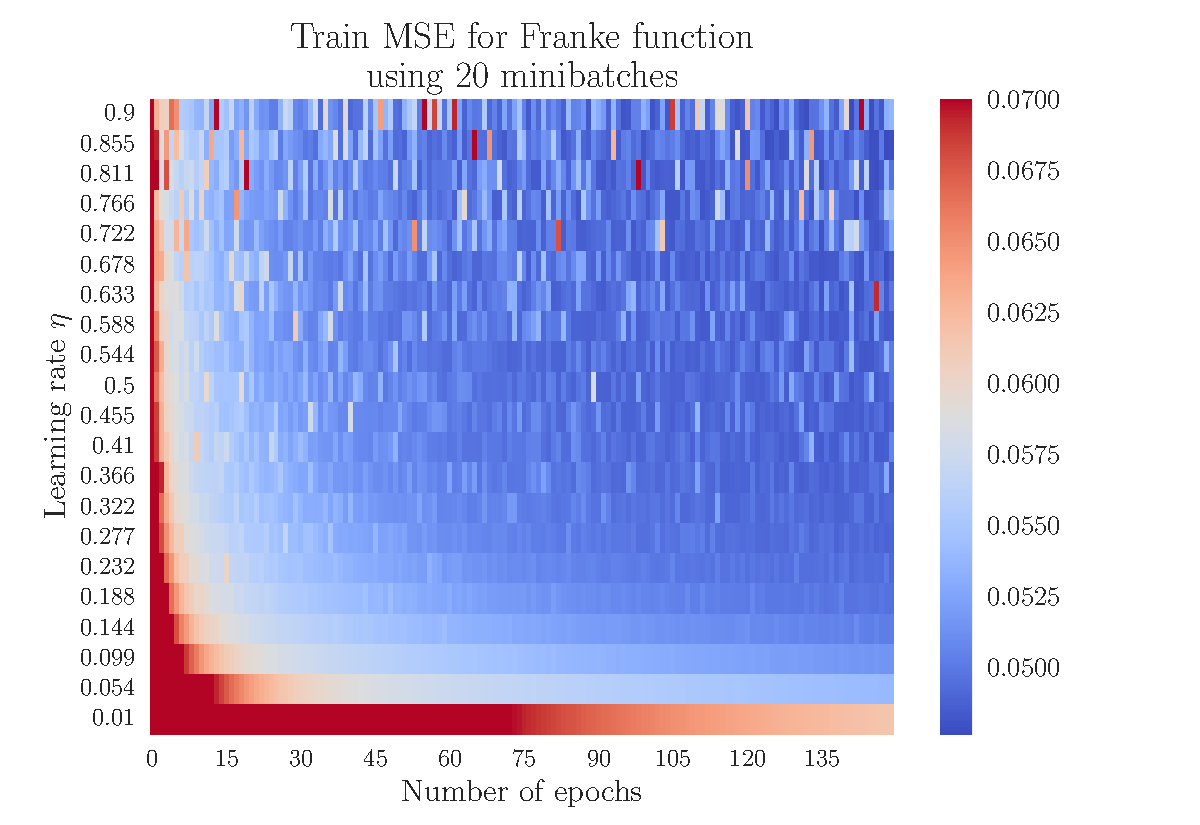
\includegraphics[width=\linewidth]{SGD_Franke/reg_Franke__epochs_eta__Train_MSE__overfit_489047.pdf}
	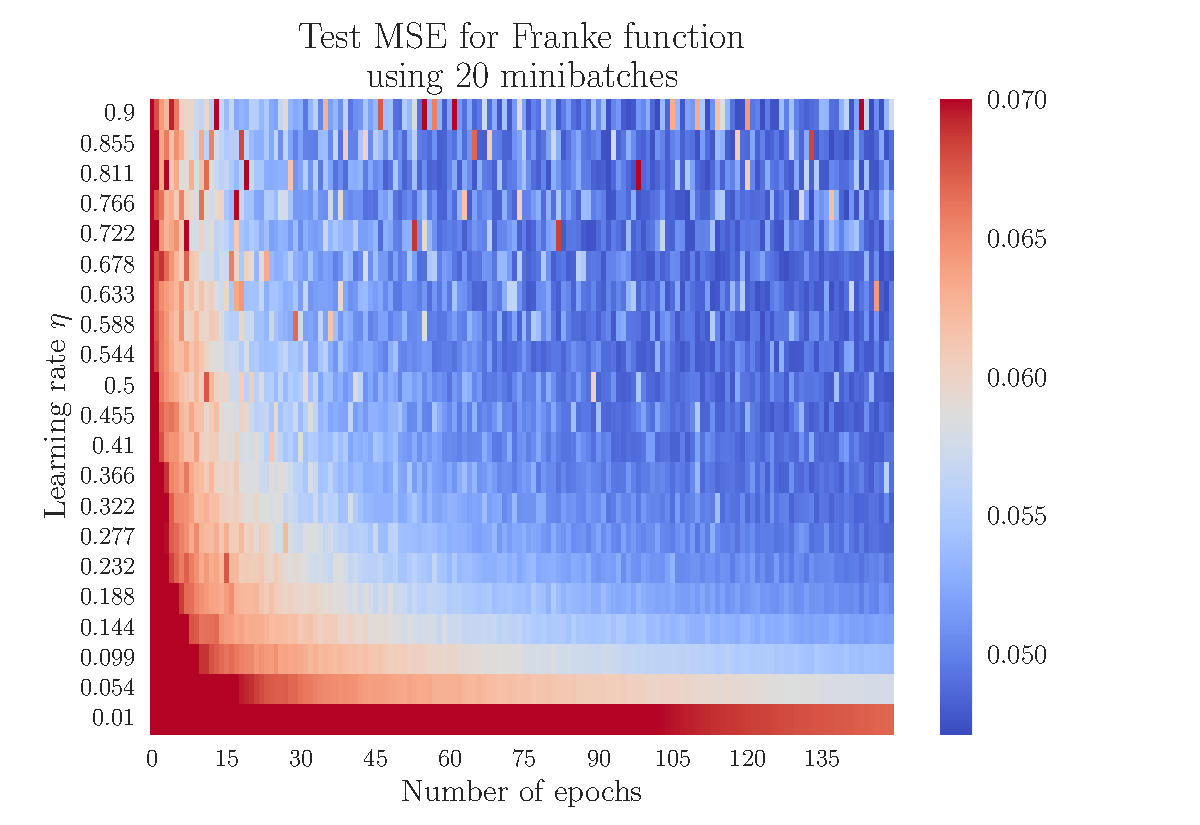
\includegraphics[width=\linewidth]{SGD_Franke/reg_Franke__epochs_eta__Test_MSE__overfit_395885.pdf}
	\caption{Initial MSE of the train and test data as a function of epochs for different learning rates $\eta$. A maximum MSE value of $0.07$ is set, so dark red regions may correspond to significantly higher MSE than it appears to.}
	\label{fig:SGD_Franke_epochs_eta_overfit}
\end{figure}

In figure \ref{fig:SGD_Franke_epochs_eta_overfit} we see that the test MSE converges faster for increased values of $\eta$ as expected. For $\eta=0.01$ we get an MSE barely below $0.07$ after $N_e=150$, as the gradient steps are too small. When $\eta$ exceeds $0.5$ we get abrupt increases of the test MSE after certain epochs. These learning rates are too high, as a gradient step goes beyond the actual minima. For $\eta=0.9$ this effect is apparent, with large fluctuations of the MSE over certain epochs.

We proceed by plotting the test MSE for $\eta\in[0.01,\,0.5]$, shown in figure \ref{fig:SGD_Franke_epochs_eta}. We clearly see how the increased learning rate yields a faster converging result, but at the expense of MSE stability, which we can see from clear fluctuations at $\eta=0.5$. When our prediction approaches the desired model, the gradients are relatively small, such that high learning rates potentially overshoots minima.

\begin{figure}[h!]
	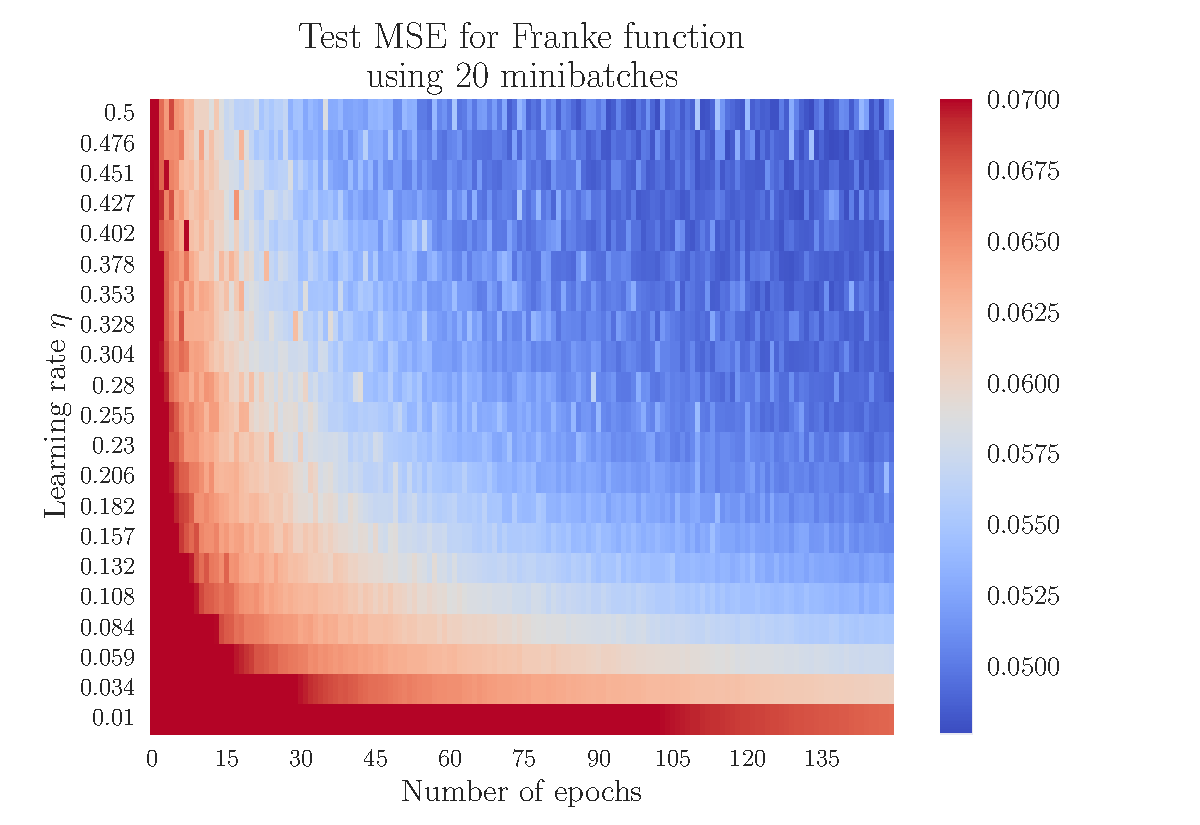
\includegraphics[width=0.9\linewidth]{SGD_Franke/reg_Franke__epochs_eta__Test_MSE__262224.pdf}
	\caption{Test MSE for different $\eta$ values. $\eta<0.25$ gives a relatively slowly converging MSE, while $\eta>0.25$ gives fluctuating MSE values. Maximum MSE$=0.07$ is chosen.}
	\label{fig:SGD_Franke_epochs_eta}
\end{figure}

When studying different number of minibatches and momentum parameters $\gamma$, we will choose a specific $\eta$. Looking at figure \ref{fig:SGD_Franke_epochs_eta}, although there are many candidates, $\eta=0.25$ yields fairly quick convergence of the MSE without significant variations. This choice appears to lie near a boundary between slow convergence and minima overshooting, and when testing other parameters we are more likely to encapsulate both cases at once.

The MSE as a function of epochs for different number of minibatches is shown in figure \ref{fig:SGD_Franke_epochs_minibatches}. We notice that by using too few minibatches, we converge more slowly. When we use $N_B=30$ we get a quickly converging MSE with a low minimum value, but there appears to some fluctuations. Because of the small batch size, the batches are more prone to consist of points not giving a good approximation of the gradient.

\begin{figure}[h!]
	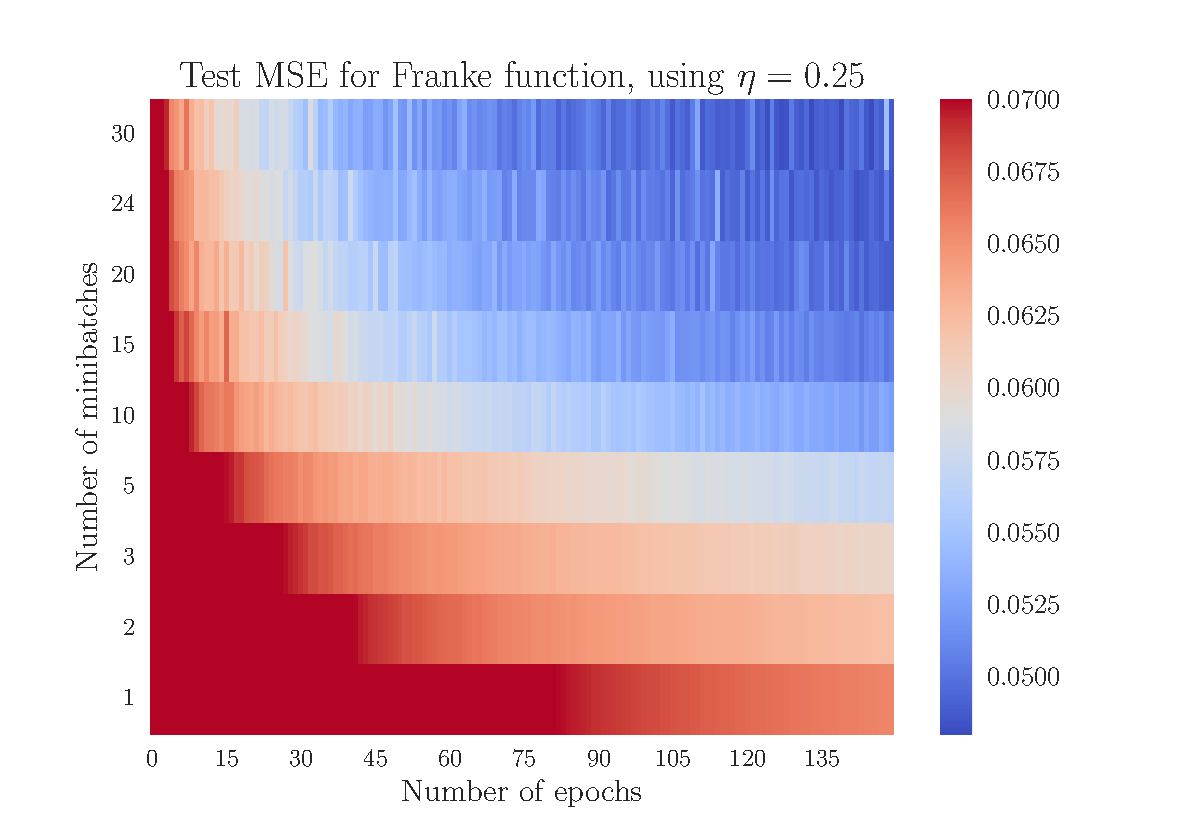
\includegraphics[width=0.9\linewidth]{SGD_Franke/reg_Franke__epochs_minibatches__Test_MSE__440533.pdf}
	\caption{Test MSE for different number of minibatches. The bottom line corresponds to no minibatches overall, and clearly gives the worst result. The heatmap is produced with $\mathrm{MSE}_\mathrm{max}=0.07$.}
	\label{fig:SGD_Franke_epochs_minibatches}
\end{figure}

We plot the test MSE after $N_e=150$ epochs with different regularization parameters in figure \ref{fig:SGD_Franke_lambda_eta}. Using the same $\eta$ interval as before and $\lambda\leq1$ we do not set an upper limit on the shown MSE, as we are interested in the general impact of the $\lambda$ values, and not nuances of the lowest values. We see in the figure that the results are not very affected by the choice of $\eta$. However, the MSE is lowest for small values of $\lambda$, increasing quickly for higher $\lambda$ values. This is similar to what we saw with linear regression \cite{project1}, though we then observed a small dip in the MSE for $\log10(\lambda)=-2.07$ for certain polynomial degrees.


\begin{figure}[h!]
	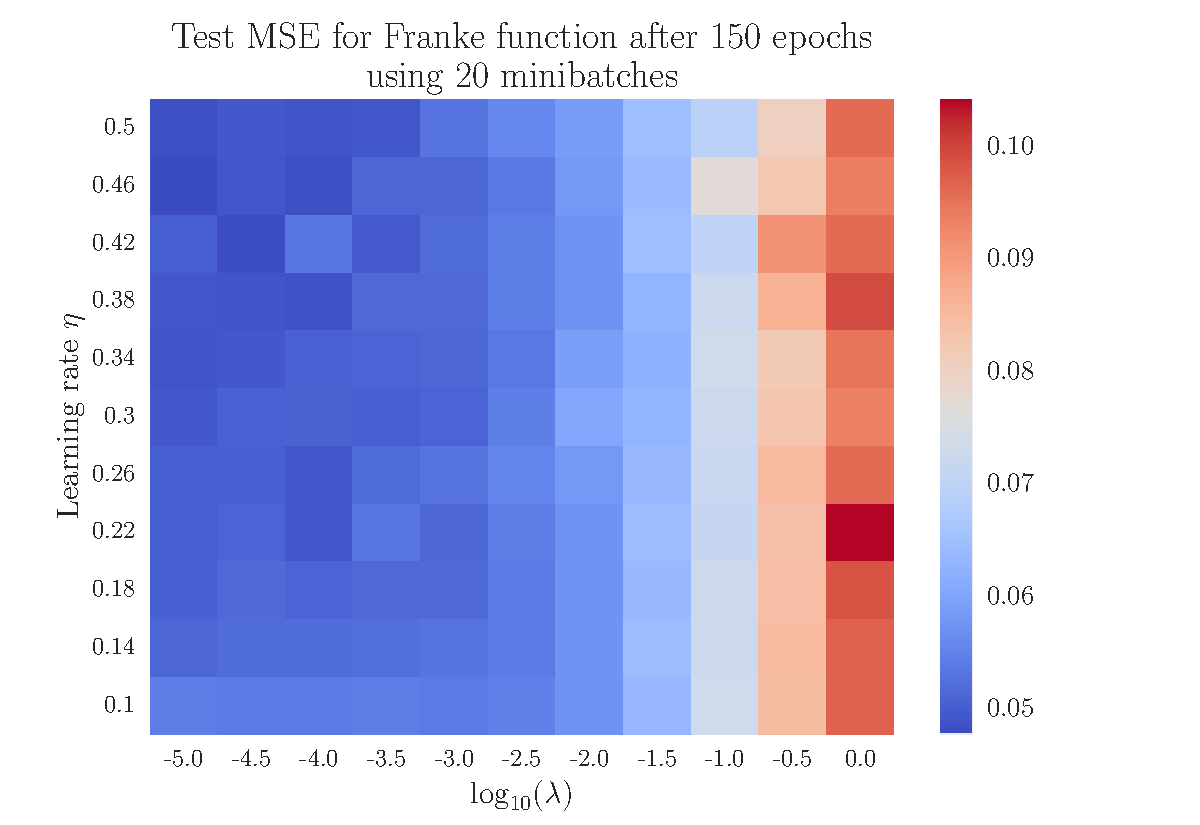
\includegraphics[width=0.9\linewidth]{SGD_Franke/reg_Franke__lambda_eta__Test_MSE__764274.pdf}
	\caption{MSE for different values $\lambda$, corresponding to Ridge regression, for different $\eta$ values.}
	\label{fig:SGD_Franke_lambda_eta}
\end{figure}


Figure \ref{fig:SGD_Franke_epochs_gamma} shows the resulting MSE values for the test data with different momentum parameters as a function of $N_e\in[0,\,150]$. We see that increasing $\gamma$ values causes the MSE to drop faster, particularly in the beginning when the gradients are large, which is expected. We also notice that $\gamma\gtrsim0.35$ results in fluctuations of the MSE, especially evident for $\gamma=0.7$, where it appears that step sizes taken following large gradient values are too big. It appears that $\gamma=0.2$ is the optimal value for this particular test, as it is small enough to avoid overshooting minima for high gradients, while still increasing the convergence rate.

\begin{figure}[h!]
	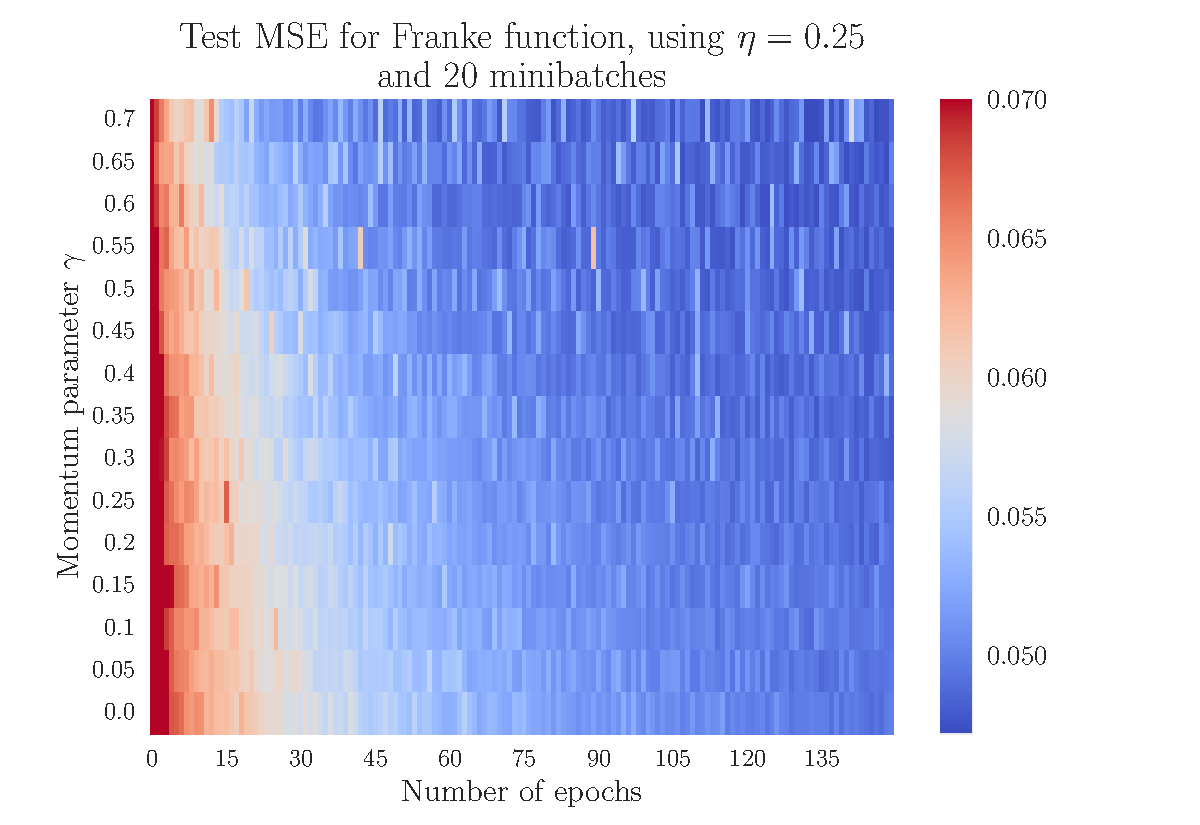
\includegraphics[width=0.9\linewidth]{SGD_Franke/reg_Franke__epochs_gamma__Test_MSE__239373.pdf}
	\caption{MSE evolution for different momentum parameters, using $\mathrm{MSE}_\mathrm{max}=0.07$, as before. The bottom line corresponds to no momentum.}
	\label{fig:SGD_Franke_epochs_gamma}
\end{figure}

The MSE calculated with dynamic $\eta$ is shown in figure \ref{fig:SGD_Franke_epochs_dynamic_eta}, using $\eta_0\in[0.1,\,0.9]$. We include the $\eta$ values previously found to be too high, in order to see whether the scheduled learning gives better results here, while omitting values of $\eta<0.1$. The figure gives us the expected result that high initial values of $\eta$ no longer causes abrupt variations of the MSE towards the end of the simulation, as $\eta\to0$ and $N_e\to150$. Equation \eqref{eq:learning_schedule} appears to be a very good choice for scaling the learning rate when doing SGD, since all values of $\eta_0>0.5$ gives decent results after $150$ epochs. These solutions converge quickly in the beginning, and as the learning rate drops we get very stable evolutions of the MSE, with no apparent instability in MSE. It appears however that the learning rates become so small towards the end that there is little evolution of the MSE after $120$ epochs, meaning that we might not actually have reached an optimal MSE score if the small learning rates near the end have effectively halted convergence. Further, the dynamic learning schedule gives more or less identical MSE values in the end for $\eta_0>0.5$. The advantage of this is that our model is less dependent on very specific parameter choices for $\eta$. If however, the final result is inadequate, adjusting the initial learning rate will no longer have a desired impact. More training epochs is then required to get optimal results.

\begin{figure}[h!]
	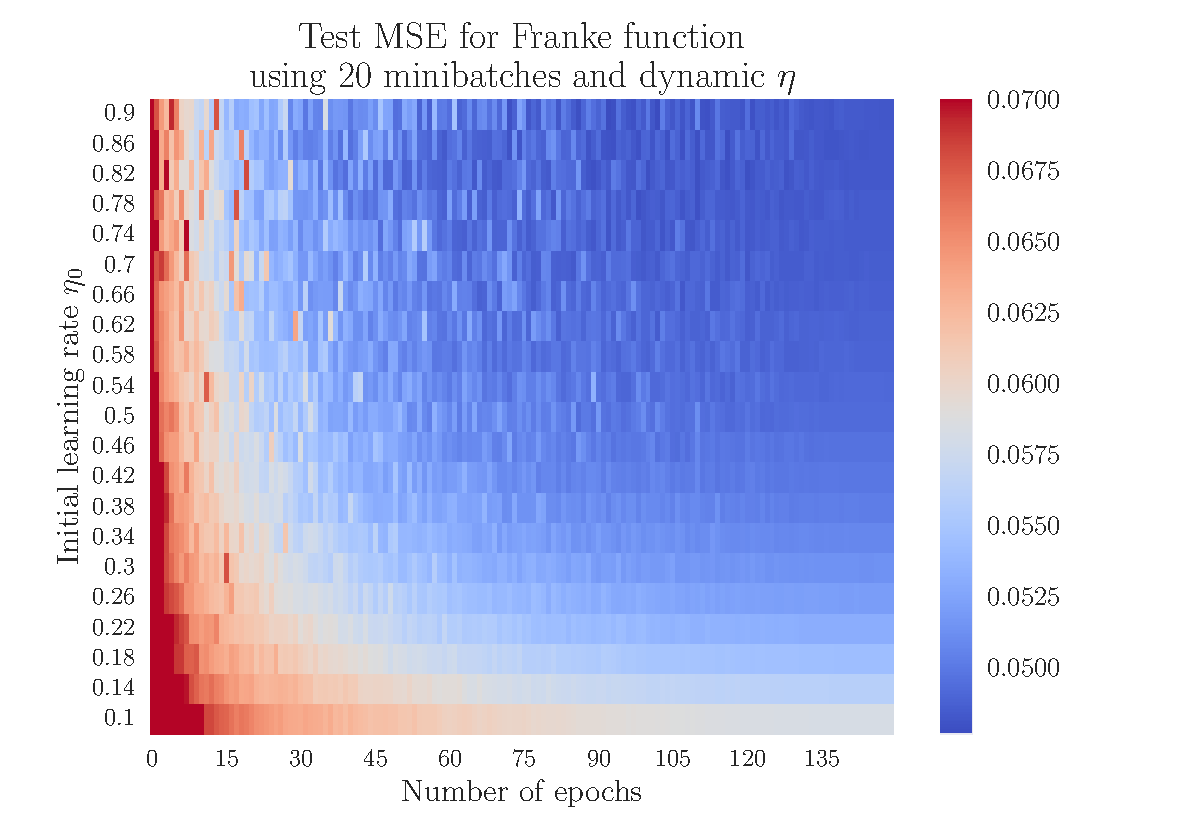
\includegraphics[width=0.9\linewidth]{SGD_Franke/reg_Franke__epochs_dynamic_eta__Test_MSE__792536.pdf}
	\caption{Evolution of the MSE for different values of $\eta_0$, all of them decreasing linearly to a final value of $\eta=0$ after $150$ epochs.}
	\label{fig:SGD_Franke_epochs_dynamic_eta}
\end{figure}


\subsubsection{Feed Forward Neural Network}

We plot the train MSE of the Franke function for different learning rates as a function of epochs, shown in figure \ref{fig:NN_Franke_epochs_eta_MSE}. We do not cap the upper limit of the MSE. We get a clear indication of good choices of $\eta$, as where it is too high or low our network does not converge. The corresponding plot for test is not shown, but was very similar, with slightly higher MSE, as expected. We will in the following figures cap the MSE at $0.07$, like what was done for SGD.

\begin{figure}[h!]
	% \minipage{0.49\textwidth}
	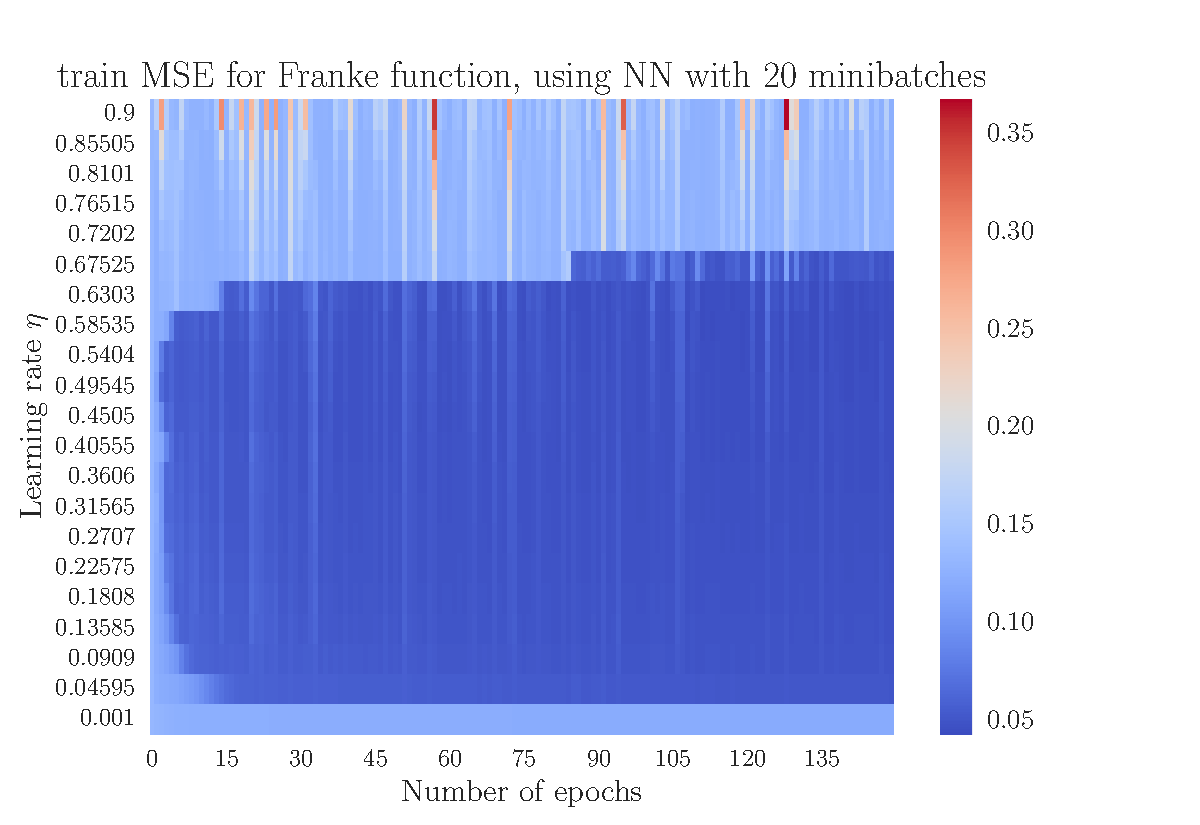
\includegraphics[width=\linewidth]{NN_Franke/NN_Franke__epochs_eta__train_MSE__569887.pdf}
	% \endminipage
	% \minipage{0.49\textwidth}
	% 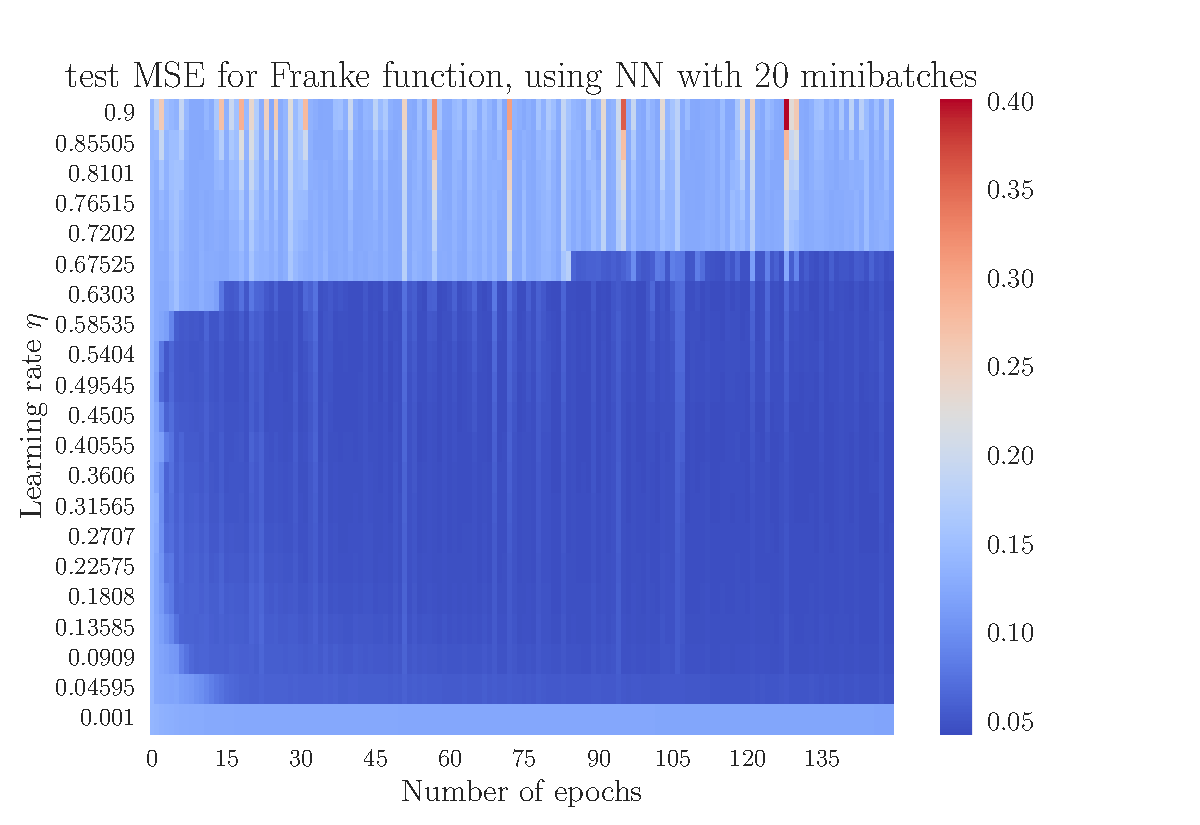
\includegraphics[width=\linewidth]{NN_Franke/NN_Franke__epochs_eta__test_MSE__271070.pdf}
	% \endminipage
	\caption{MSE of the train data during $150$ epochs for different learning rates using a Neural network.}
	\label{fig:NN_Franke_epochs_eta_MSE}
\end{figure}


We choose $\eta\in[0.05,\,0.5]$ and plot the test MSE as a function of $N_e=250$ epochs shown in figure \ref{fig:NN_Franke_epochs_eta_MSE_limited}. The figure shows how the MSE drops as we continue to train the network, with little evidence of overfitting, which would be a general increases of the MSE towards the end of training. We do however see some clear vertical lines; abrupt increases of the MSE for all $\eta$. These were not expected, though can possibly be explained through the way the network is trained. In order to keep results comparable over many runs, the seed of the random distribution is set before each net is created. This was mainly to ensure that the weights are initialized the same for all. However, a side effect of this is that the dataset is split into the same batches for each net, at a given epoch. Sometimes these batches lead to a bad approximation of gradient for the enitre dataset, giving worse test results. Here that happens at the same epoch every time.


\begin{figure}[h!]
	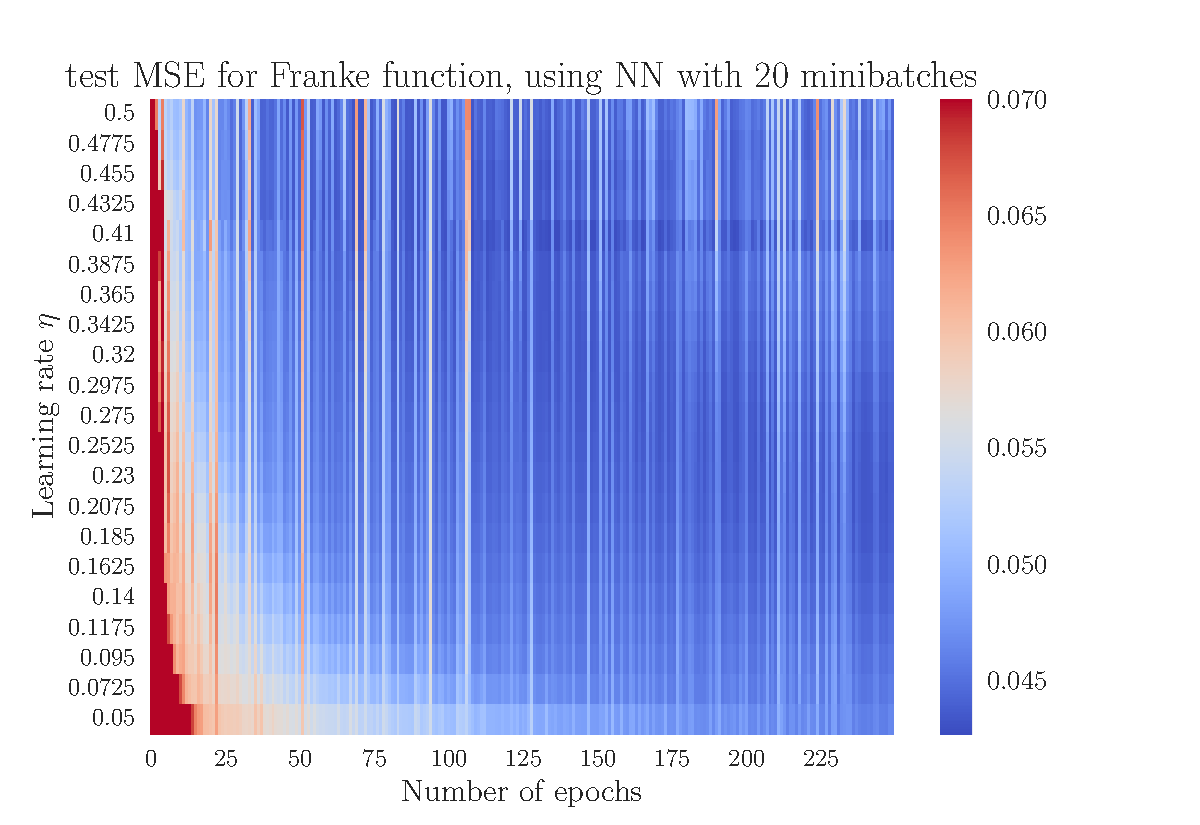
\includegraphics[width=\linewidth]{NN_Franke/NN_Franke__epochs_eta__test_MSE__582234.pdf}
	\caption{Test MSE of the Franke function for different learning rates, during training.}
	\label{fig:NN_Franke_epochs_eta_MSE_limited}
\end{figure}


We proceed by plotting the $R^2$ score, setting a minimum value of $R^2=0.55$ to highlight results in the same vicinity of what we got for linear regression in \cite{project1}, shown in figure \ref{fig:NN_Franke_epochs_eta_R2}. While in the results for MSE, red indicated bad values as we want to minimize MSE, for $R^2$, red is good, as we want it maximized. The figure shows that we obtain $R^2$ scores exceeding the ones we obtained with linear regression, where the test $R^2_\mathrm{test}<0.6$ was obtained without resampling, while we exceed this value for multiple configurations of the neural network. Other than a relative score, the $R^2$ score does not appear to provide any new information, as we got similar MSE values using linear regression. Thus, the $R^2$ figures are essentially the negatives of the MSE figures, and will not be used for further assessing our model.

\begin{figure}[h!]
	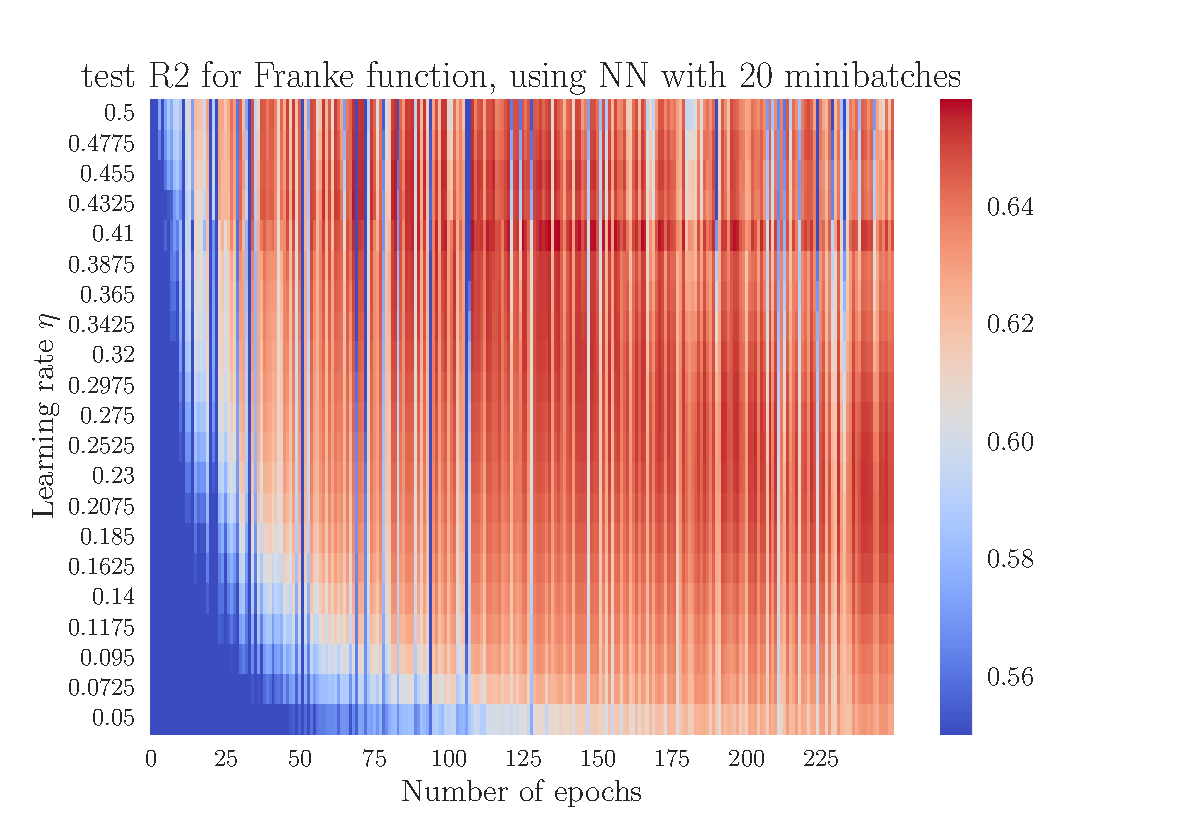
\includegraphics[width=\linewidth]{NN_Franke/NN_Franke__epochs_eta__test_R2__190748.pdf}
	\caption{The $R^2$ score of the Neural network, using a minimum value of the heatmap of $R^2_\mathrm{min}=0.55$.}
	\label{fig:NN_Franke_epochs_eta_R2}
\end{figure}

Figure \ref{fig:NN_Franke_epochs_dynamic_eta} shows the evolution of the MSE when we use dynamic learning rates, calculated with equation \eqref{eq:learning_schedule} as before. The result is similar to what we obtained with SGD, with suppressed fluctuations of the MSE for higher epochs. This has a fairly large effect on the Neural network, as the fluctuations of the MSE for $N_e>200$ in figure \ref{fig:NN_Franke_epochs_eta_MSE_limited} are no longer present. Because the learning rate goes down as function of epoch, the bad batches changes the weights less, so the abrupt increases in test MSE are gone, while the MSE is still low.

\begin{figure}[h!]
	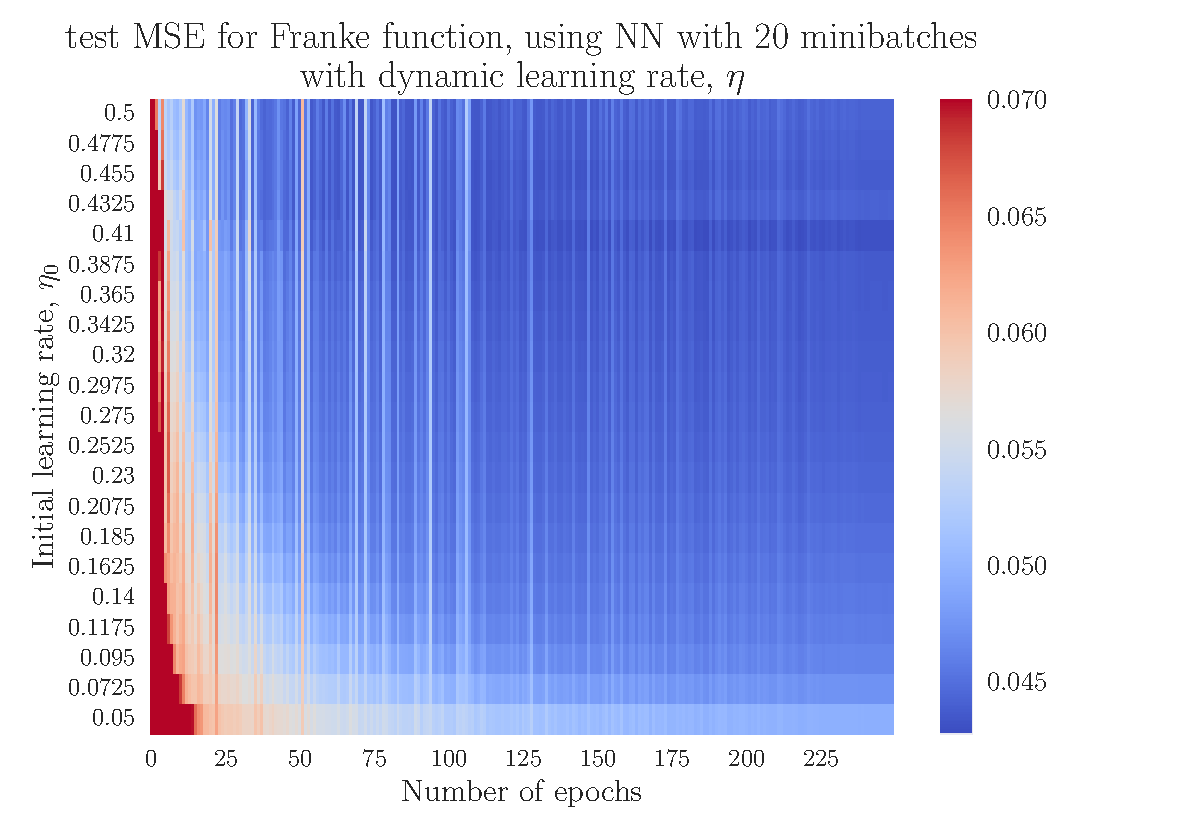
\includegraphics[width=\linewidth]{NN_Franke/NN_Franke__epochs_dynamic_eta__test_MSE__489375.pdf}
	\caption{MSE of the Franke function from the Neural network, using a linearly decreasing learning rate, where the initial learning rates are shown on the $y$-axis.}
	\label{fig:NN_Franke_epochs_dynamic_eta}
\end{figure}


Next we want to see the effects of different activation functions. We plot the test MSE over $250$ epochs using the RELU and Leaky RELU activation functions for the hidden layers, shown in the upper and lower panel of figure \ref{fig:NN_Franke_epochs_eta_MSE_relu_leaky} respectively. The dynamic $\eta$ is not used. An upper value of $0.07$ have been used for the MSE once again. Because the functions are linear for values above $0$, high activations can occur, leading to overflow. This happened for $\eta>0.15$, and thus not shown.  The difference between the two methods are not significant, as was expected, though Leaky RELU gave slightly better results. In Figure \ref{fig:NN_Franke_epochs_eta_MSE_sigmoid_compare} we show the results from sigmoid, using the same $\eta$ values. It is apparent that RELU and Leaky RELU learn much more quickly then sigmoid. While the latter needs at least 25 epochs to get a good result, the former two need 1. However, for RELU and Leaky RELU, the MSE increases again for towards the end of training for high $\eta$-values, a sign of overfitting. This indicates it is better to train those two for fewer epochs, and lower $\eta$.

\begin{figure}[h!]
	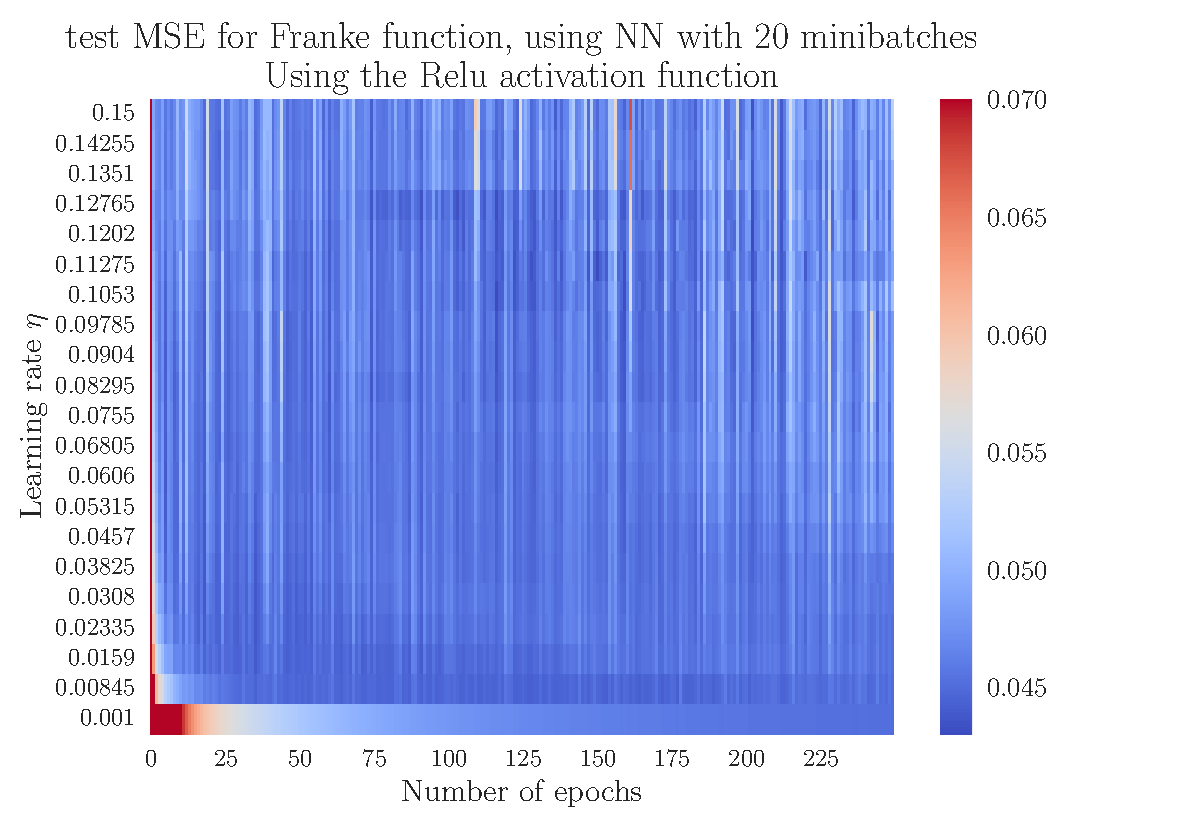
\includegraphics[width=0.8\linewidth]{NN_Franke/NN_Franke__epochs_eta__test_MSE__relu__733938.pdf}
	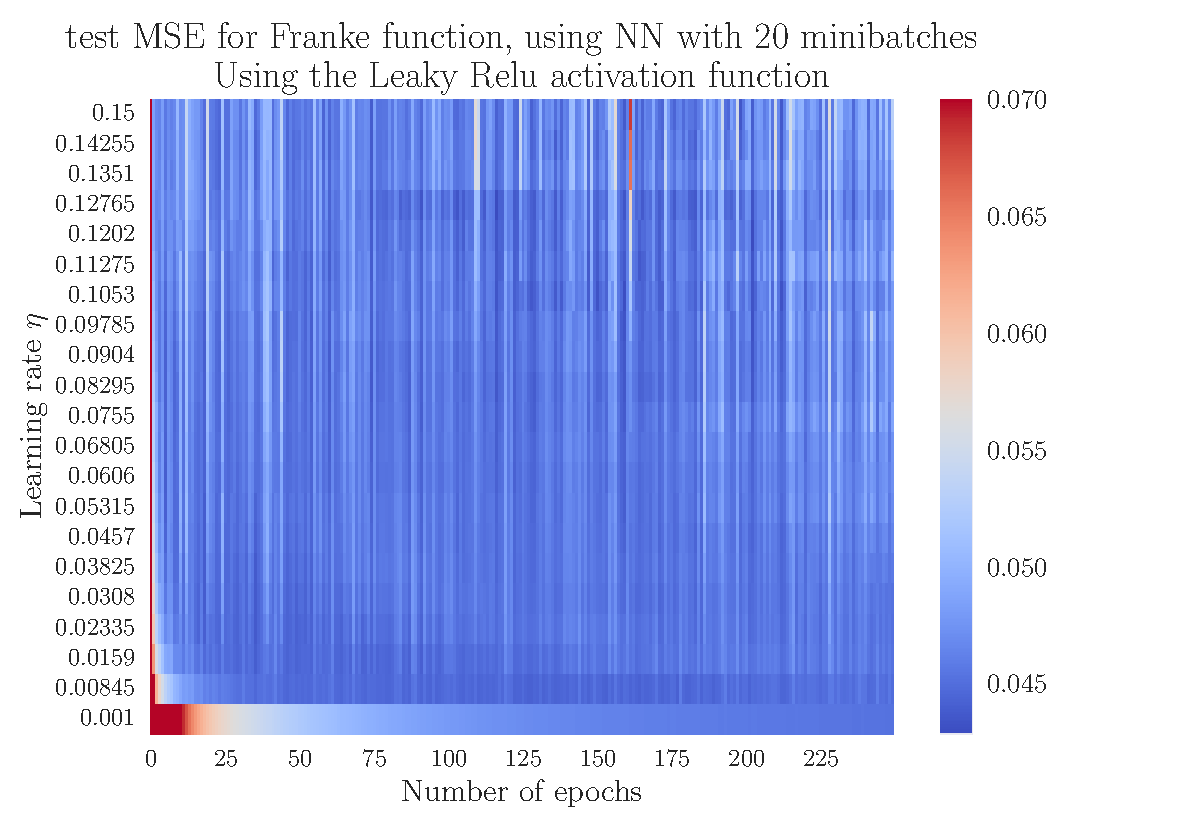
\includegraphics[width=0.8\linewidth]{NN_Franke/NN_Franke__epochs_eta__test_MSE__leaky_relu__501404.pdf}
	\caption{MSE Relu and Leaky Relu}
	\label{fig:NN_Franke_epochs_eta_MSE_relu_leaky}
\end{figure}


\begin{figure}[h!]
	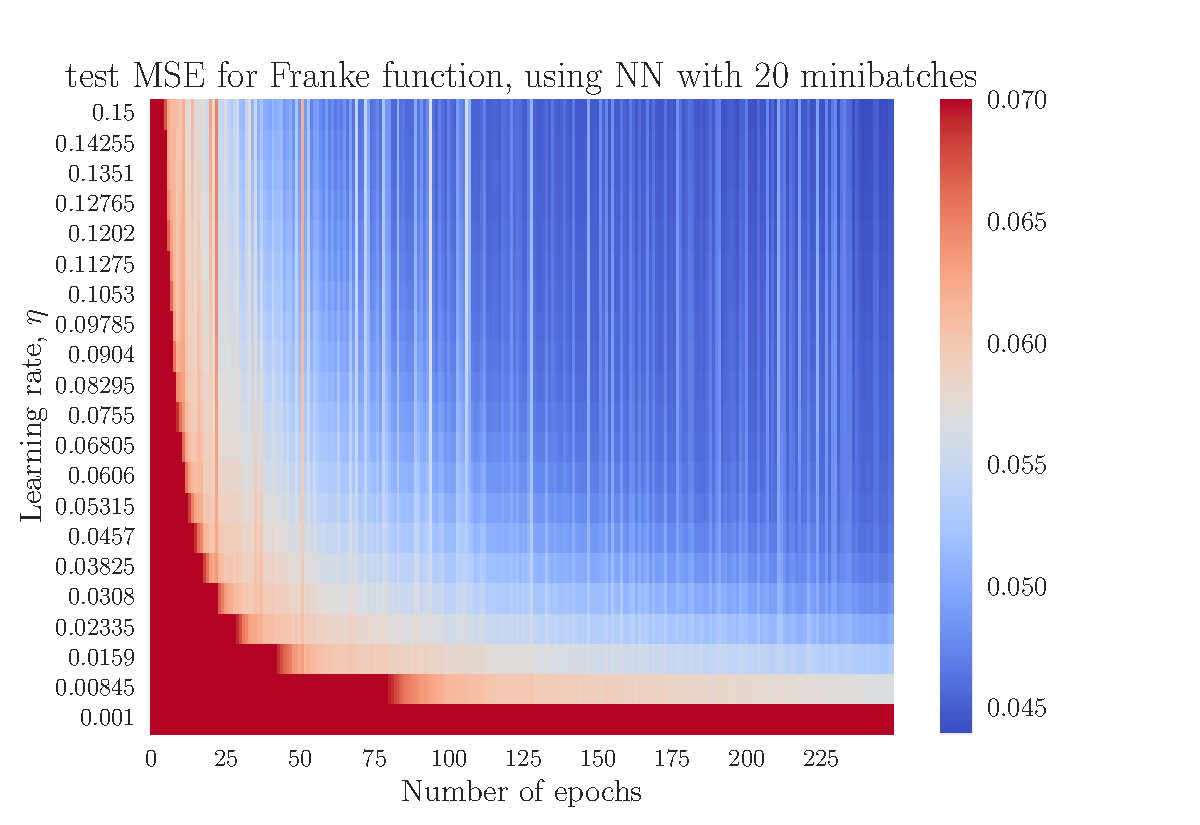
\includegraphics[width=0.7\linewidth]{NN_Franke/NN_Franke__epochs_eta__test_MSE__compare__600255.pdf}
	\caption{MSE of the Neural network with the sigmoid activation function for the hidden layers. The learning rates and epochs are identical to that of figure \ref{fig:NN_Franke_epochs_eta_MSE_relu_leaky}, allowing us to compare the effect of the different activation functions.}
	\label{fig:NN_Franke_epochs_eta_MSE_sigmoid_compare}
\end{figure}

Since a very integral part of neural networks are the neurons, we also study the way the network is structued. Until now, we have used a network with 2 hidden layers with 10 nodes in each. Without changing the total number of nodes, we train 4 networks for 100 epochs, using the activation function RELU. First, 1 (hidden) layer with 20 nodes is used. Then 2 layers with 10 each, for comparison. Then 3 layers, the middle with 10 nodes and the others with 5, and lastly 4 layers, with 5 nodes each. The same $\eta$ range as before is used. The four resulting plots are shown in Figure \ref{fig:NN_layers}. The network with 4 layers is shown in the bottom rihgt. This only learns for a very narrow range of $\eta$'s, and seems to be too deep, at least for the given value of the other parameters. The network with 3 layers, shown in the bottom left, learns slower but does reach good results. However, along with the network with 1 layer in the upper left, there is much variation. It seems the network with 2 layers perform the best, escpecially as it gives good results for a wide range of $\eta$, compared to the other networks.

\begin{figure}[h]
	\minipage{0.49\textwidth}
	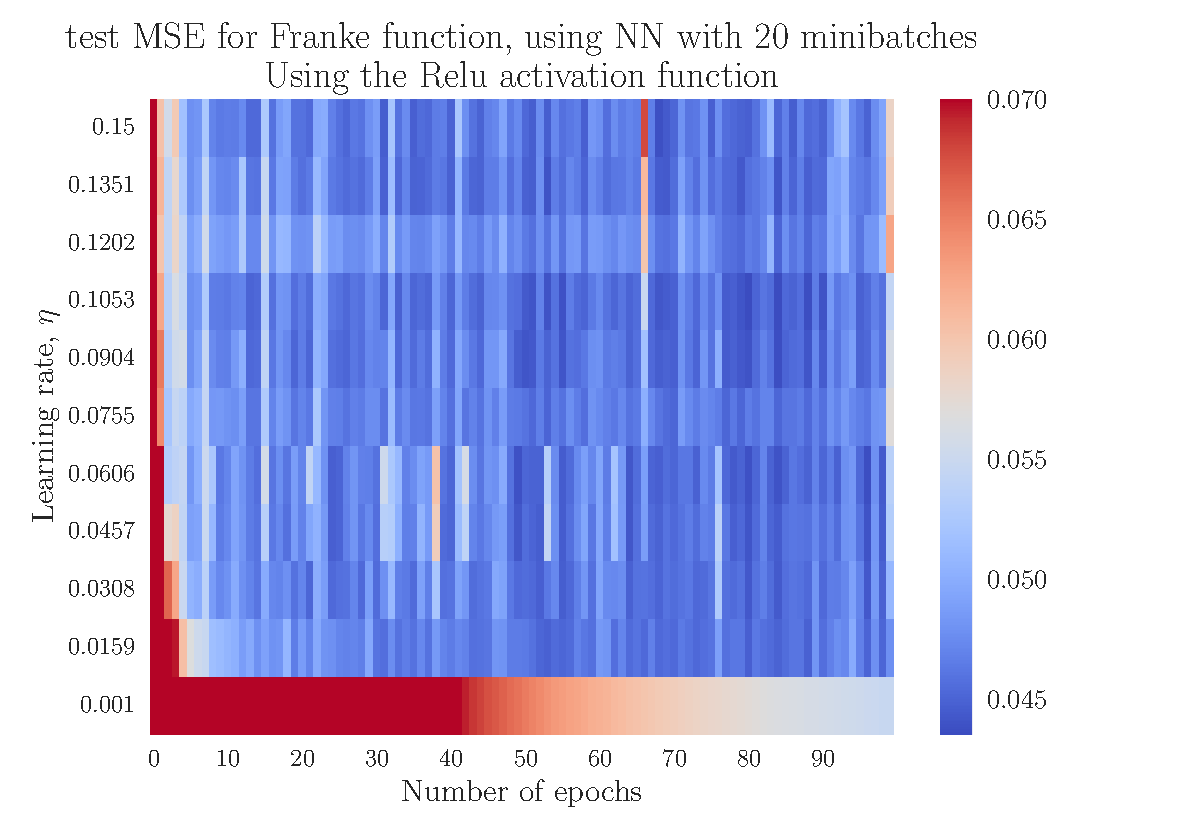
\includegraphics[width=\linewidth]{../output/plots/NN_Franke__epochs_eta__test_MSE__relu__375043.pdf}
	\endminipage\hfill
	\minipage{0.49\textwidth}
	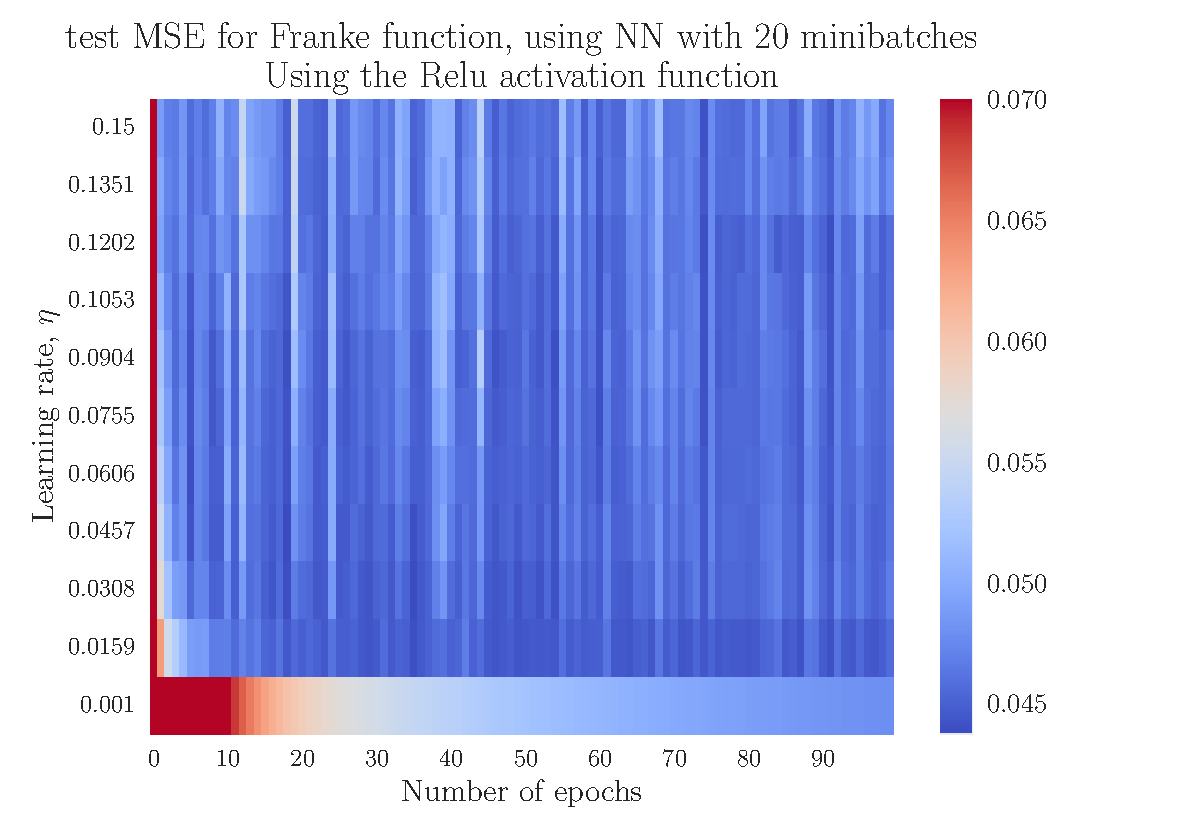
\includegraphics[width=\linewidth]{../output/plots/NN_Franke__epochs_eta__test_MSE__relu__705262.pdf}
	\endminipage\hfill
	\minipage{0.49\textwidth}
	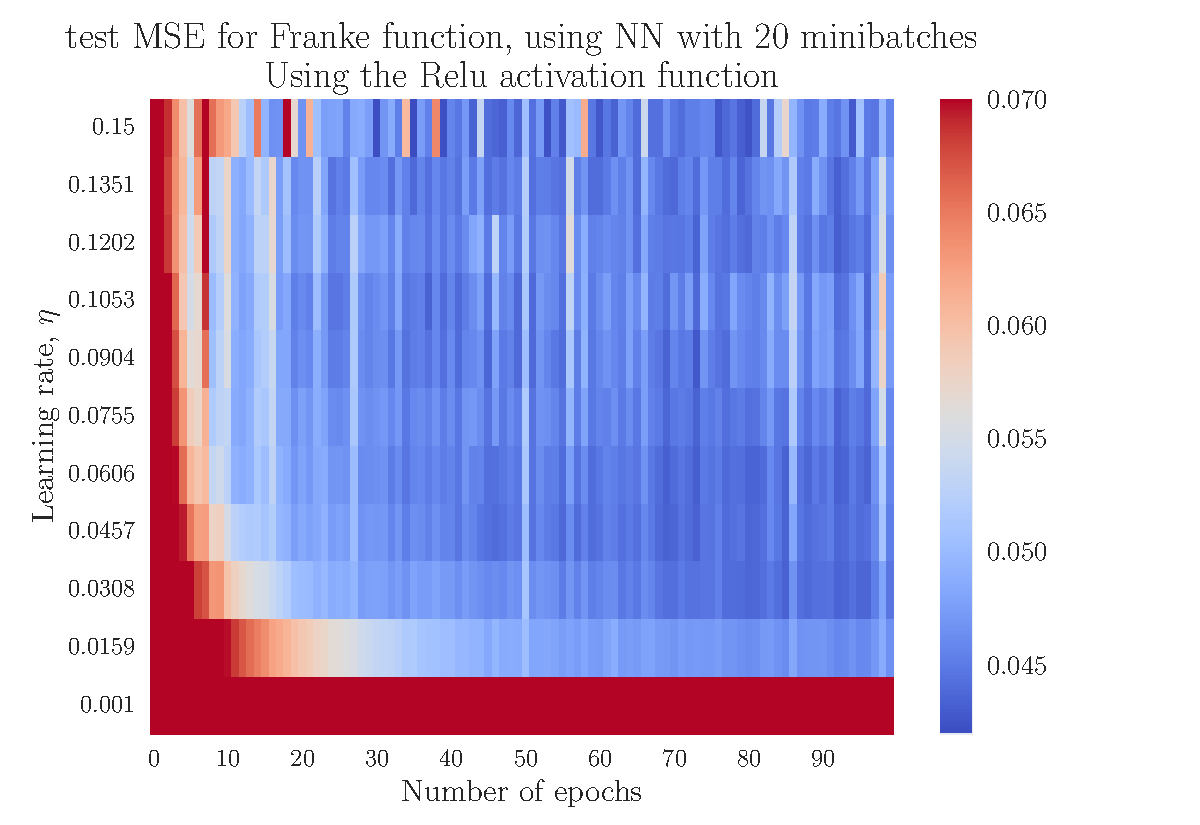
\includegraphics[width=\linewidth]{../output/plots/NN_Franke__epochs_eta__test_MSE__relu__45014.pdf}
	\endminipage\hfill
	\minipage{0.49\textwidth}
	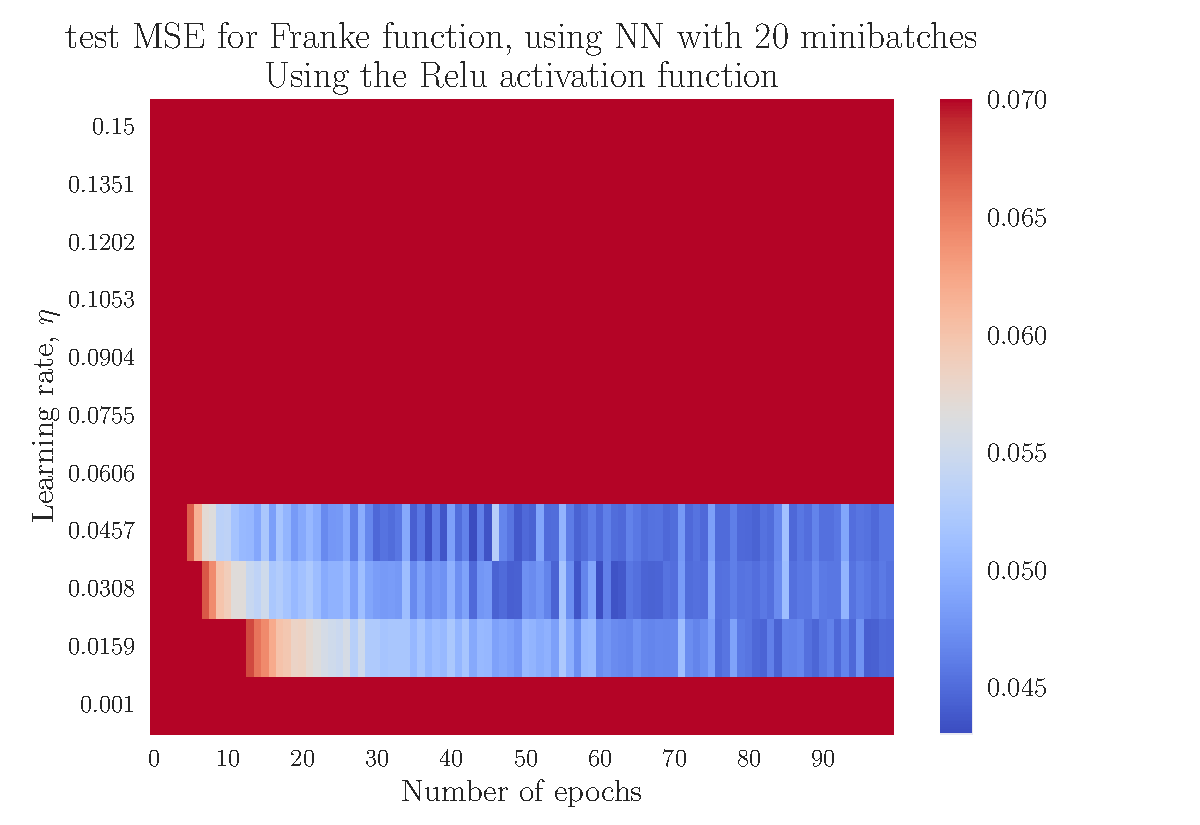
\includegraphics[width=\linewidth]{../output/plots/NN_Franke__epochs_eta__test_MSE__relu__704482.pdf}
	\endminipage
	\caption{Neural networks with different number of layers, but same number of total nodes. Top left has 1 hidden layer, top right has 2. Bottom left has 3, while bottom right has 4. All have a total of 20 nodes.}\label{fig:NN_layers}
\end{figure}

Lastly, we study the regularization parameter $\lambda$. Using the same $\eta$ values as in Figure \ref{fig:NN_Franke_epochs_eta_MSE_limited}, and sigmoid as the activation function, we plot the test MSE after 100 epochs for 15 logarithmically distributed values of $\lambda$ between $10^{-7}$ and $1$. This is shown in Figure \ref{fig:NN_lambda}. We see that we get better result for lower $\lambda$, strictly. In \cite{project1} we saw that the $\lambda$ parameters was useful if the noise in the data was higher. We made a similar figure, with $\epsilon=0.5$. The resulting MSE was (naturally) higher, but the trend was the same as seen here. We see no benefit using other values than $\lambda=0$. Other parameters or datasets could change this.


\begin{figure}[h]
	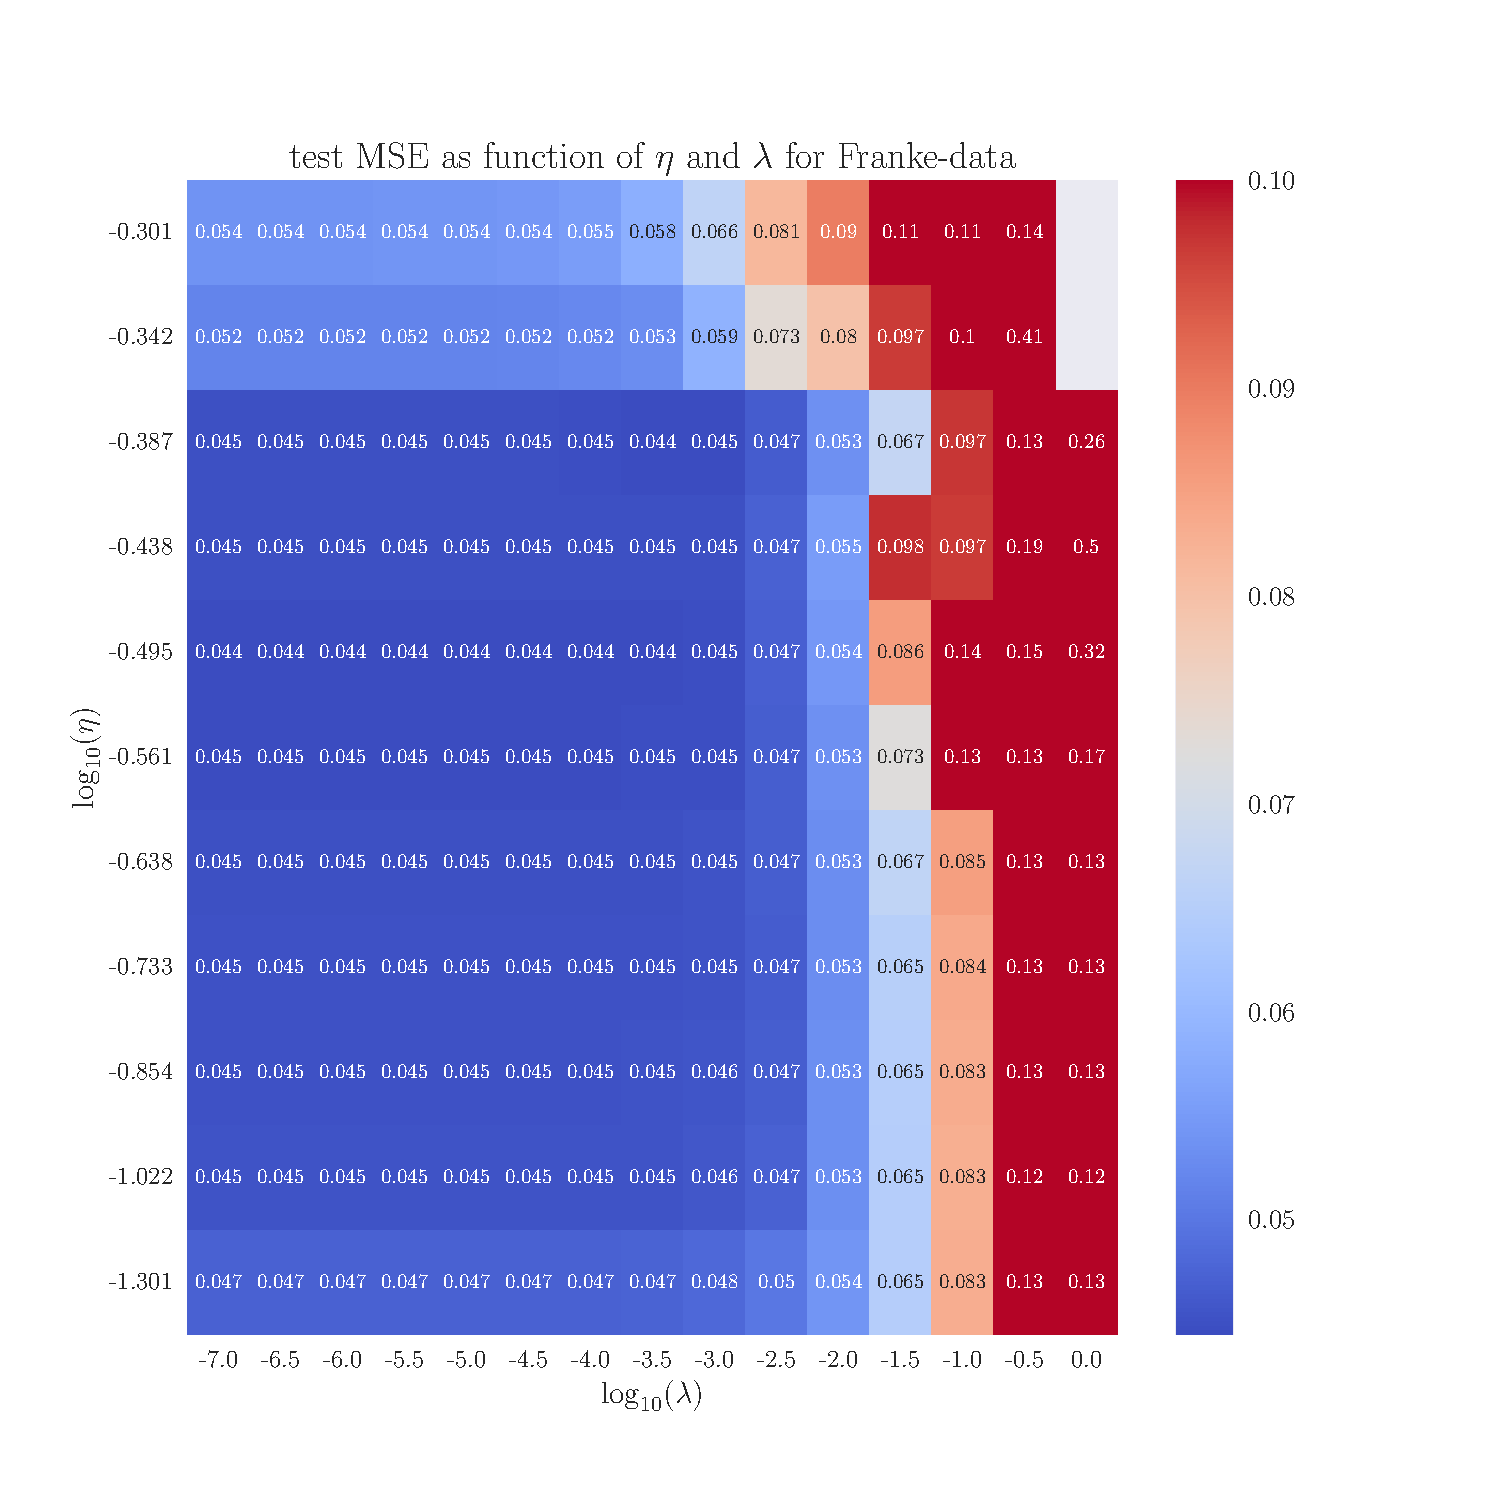
\includegraphics[width=\linewidth]{plots/NN_Franke__eta_lambda__test_MSE__228448.pdf}
	\caption{Test MSE as function of learning rate $\eta$ and regularization parameter $\lambda$. The two blank squares in the top right corner correspond to MSE higher than 1, and thus not shown.}\label{fig:NN_lambda}
\end{figure}


\clearpage
\subsection{Wisconsin Breast Cancer Data}
\subsubsection{Feed Forward Neural Network}


In Figure \ref{fig:NN_Cancer_sigmoid_dynam_eta}, we make the same plot, now using the learning schedule in equation \eqref{eq:learning_schedule}.

\begin{figure}[h]
	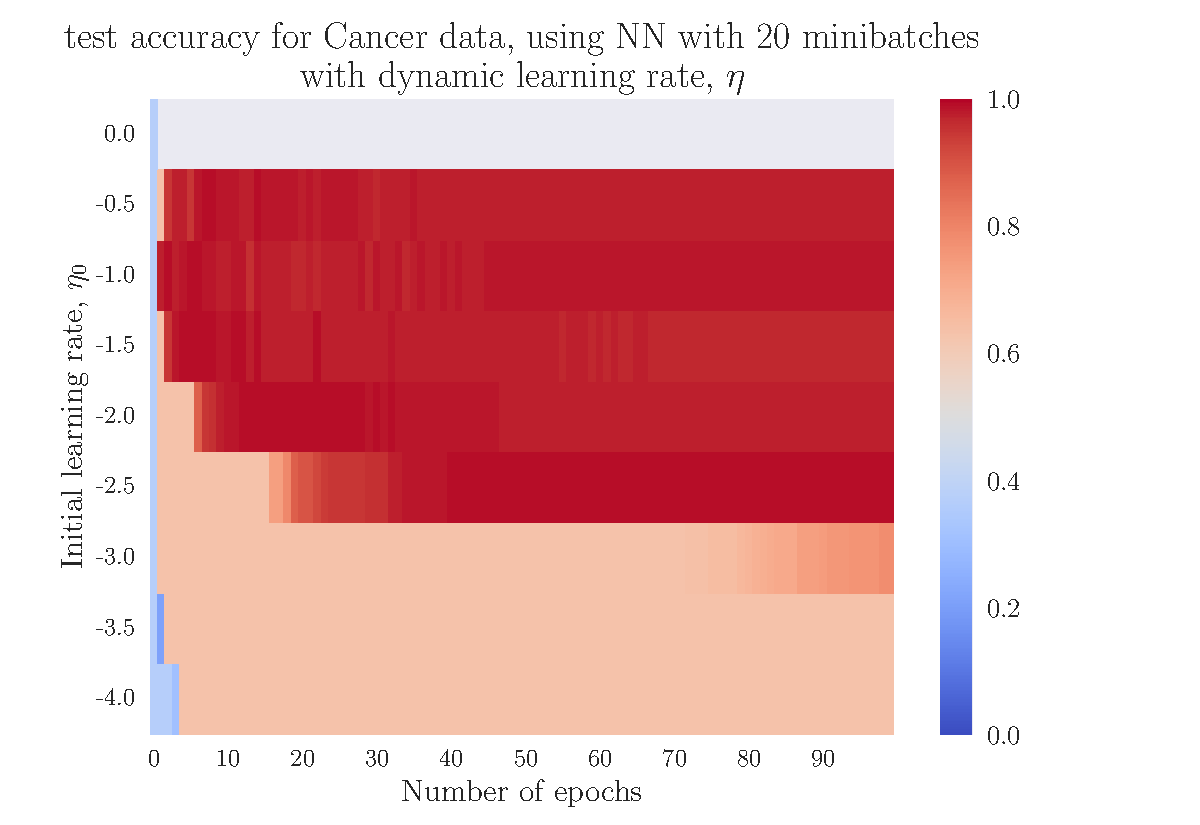
\includegraphics[width=\linewidth]{plots/NN_Cancer__epochs_dynamic_eta__test_accuracy__354289.pdf}
	\caption{Test accuracy using sigmoid as the activation function, with dynamic learning rate. For $\eta=1$, we get overflow, so no value is shown. }\label{fig:NN_Cancer_sigmoid_dynam_eta}
\end{figure}

Now we use the other implemented activation functuions

\begin{figure}[h]
	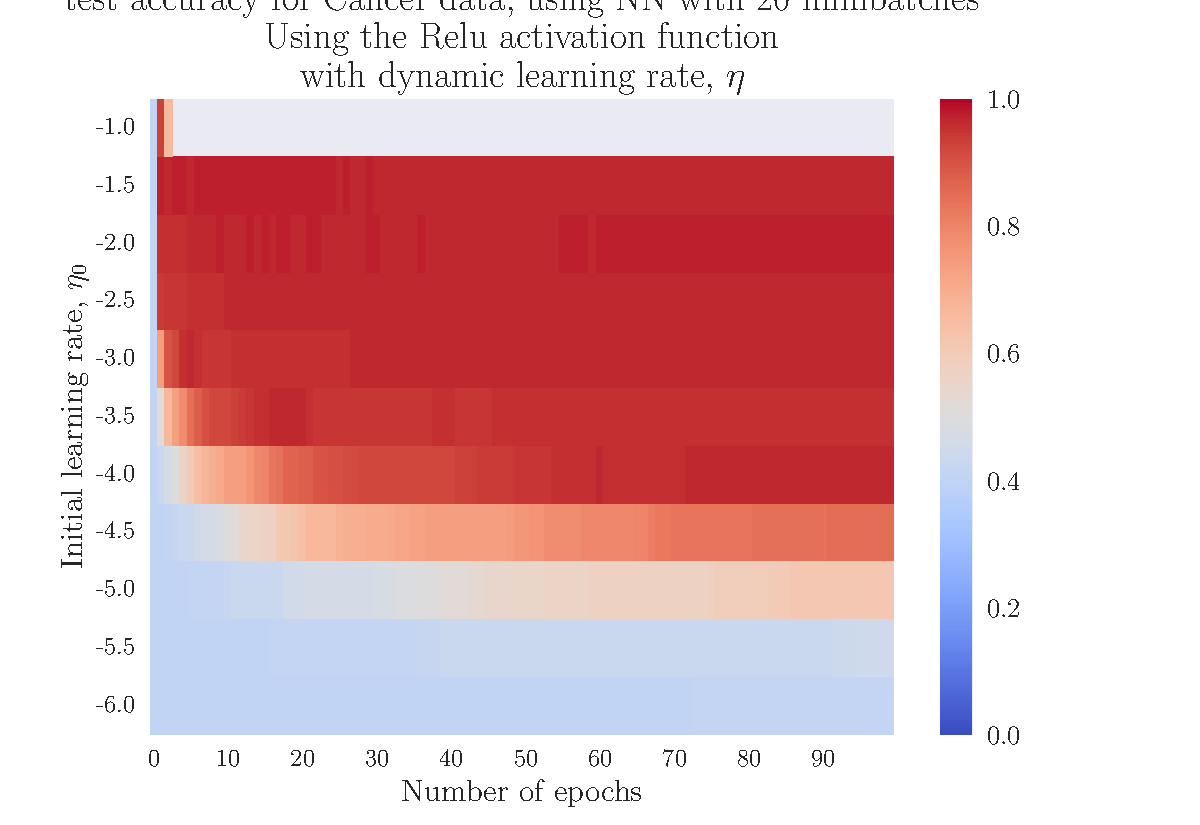
\includegraphics[width=0.5\linewidth]{plots/NN_Cancer__epochs_dynamic_eta__test_accuracy__relu__256821.pdf}
	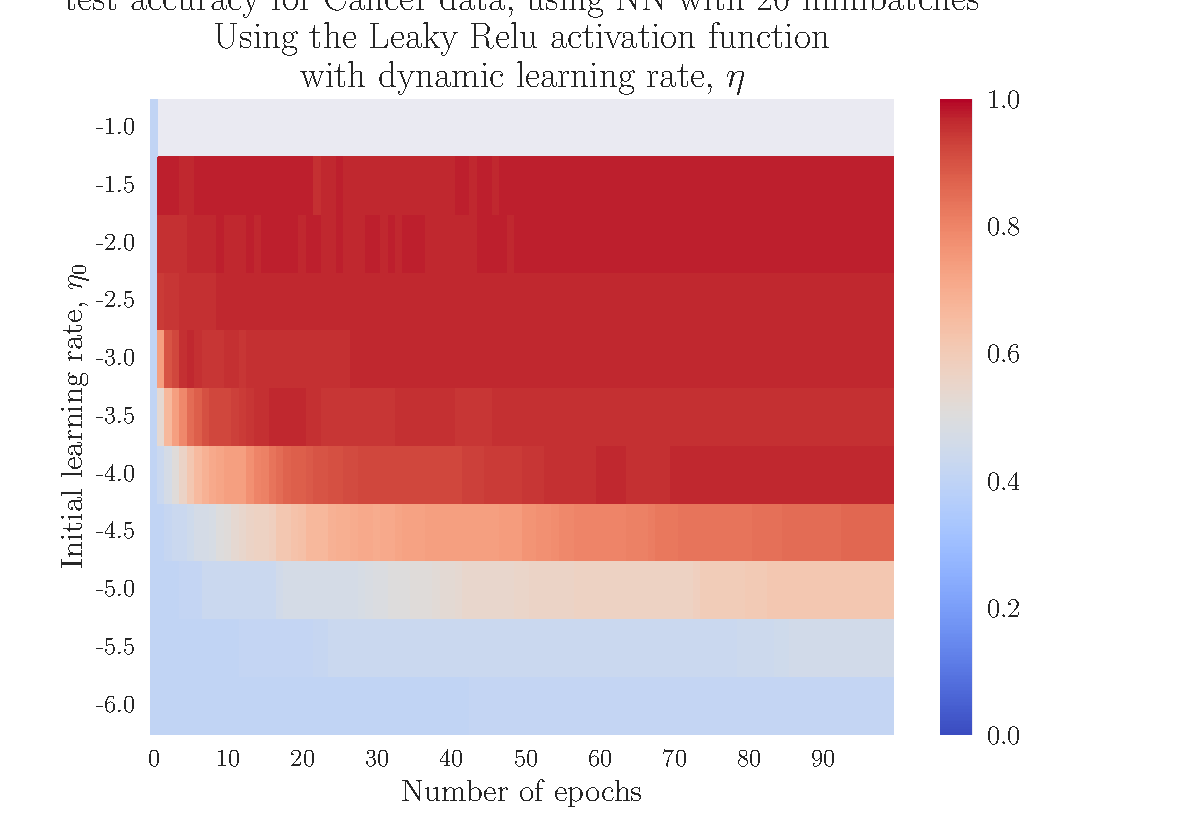
\includegraphics[width=0.5\linewidth]{plots/NN_Cancer__epochs_dynamic_eta__test_accuracy__leaky_relu__415455.pdf}
	\caption{Test accuracy using sigmoid as the activation function, with 2 hidden layers with 10 nodes each. For $\eta=1$, we get overflow, so no value is shown. }\label{fig:NN_Cancer_relu_leaky}
\end{figure}


\begin{figure}[h]
	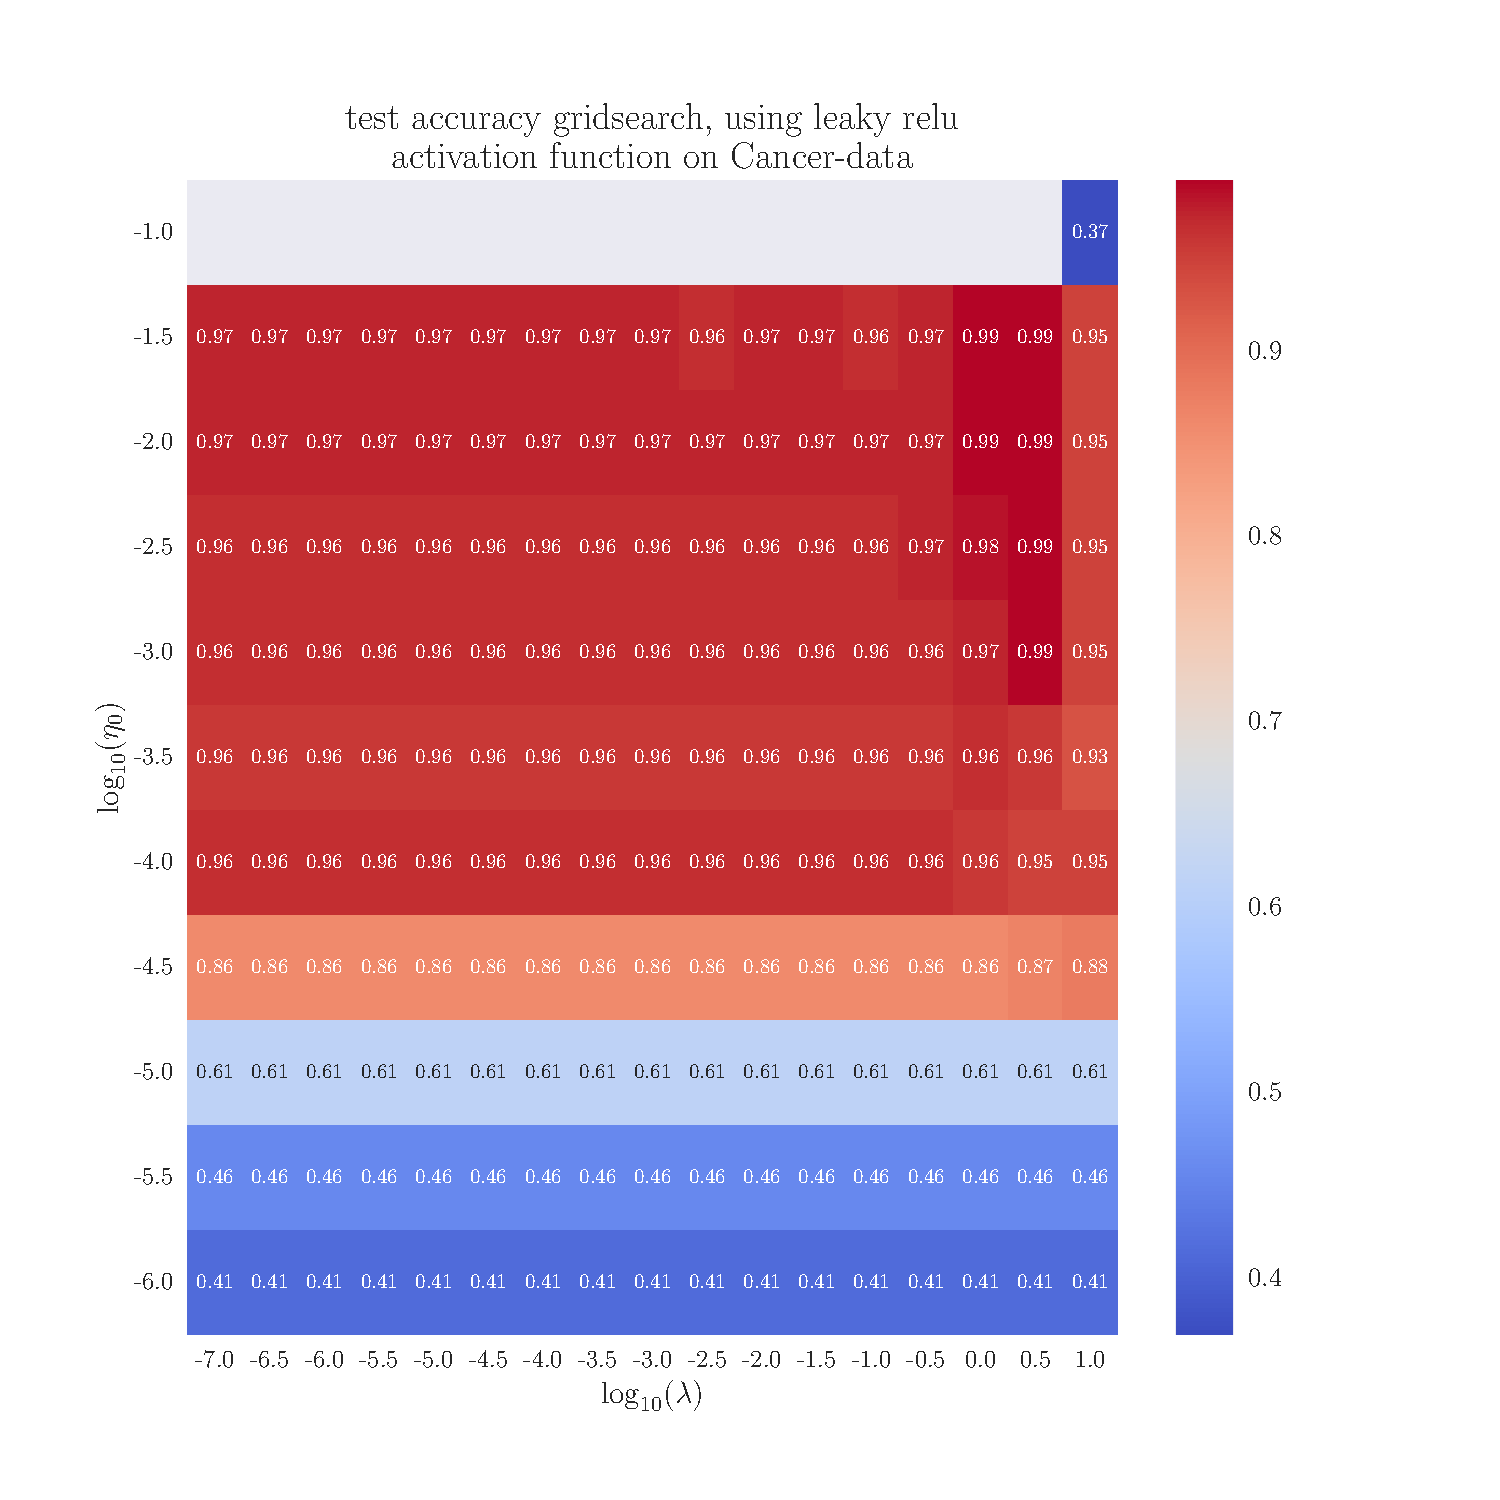
\includegraphics[width=\linewidth]{plots/NN_Cancer__dynamic_eta_lambda__test_accuracy__leaky_relu__888173.pdf}
	\caption{Test accuracy using sigmoid as the activation function, with 2 hidden layers with 10 nodes each. For $\eta=1$, we get overflow, so no value is shown. }\label{fig:NN_Cancer_eta_lambda}
\end{figure}

\begin{figure}[h]
	\minipage{0.49\textwidth}
	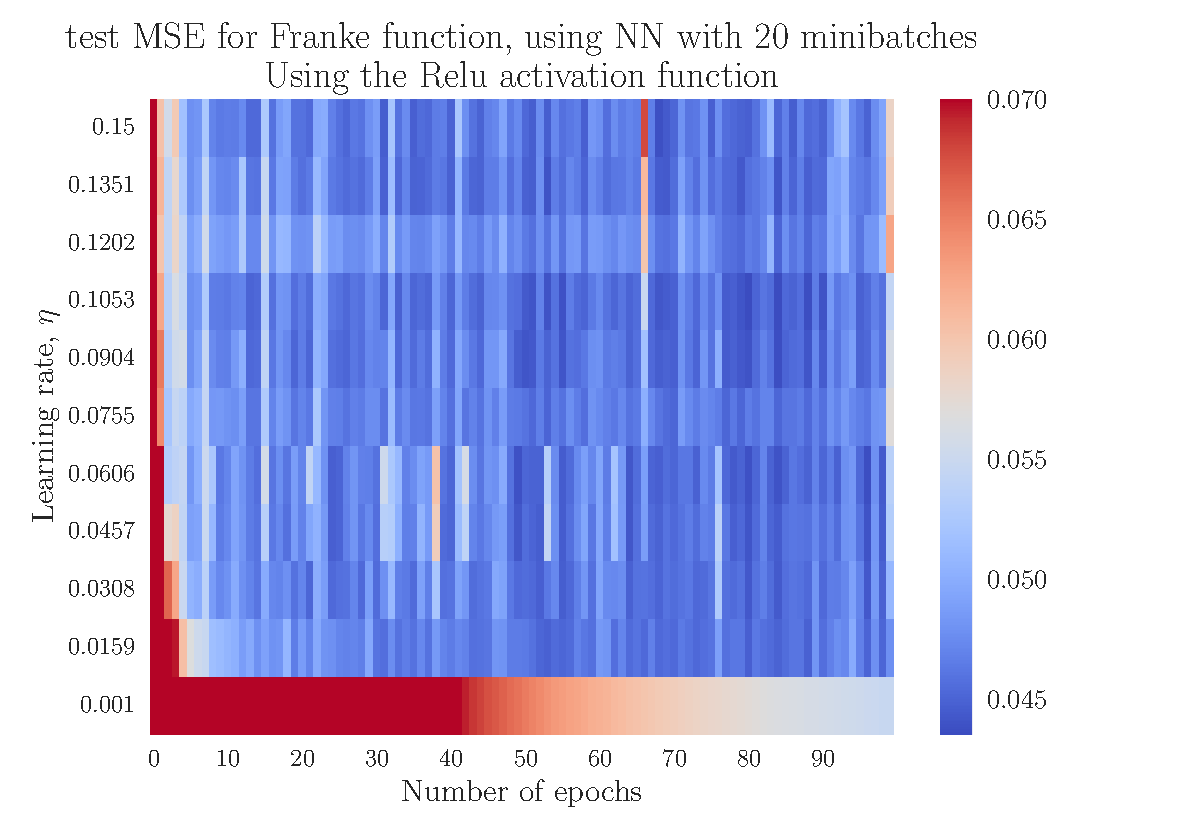
\includegraphics[width=\linewidth]{../output/plots/NN_Franke__epochs_eta__test_MSE__relu__375043.pdf}
	\endminipage\hfill
	\minipage{0.49\textwidth}
	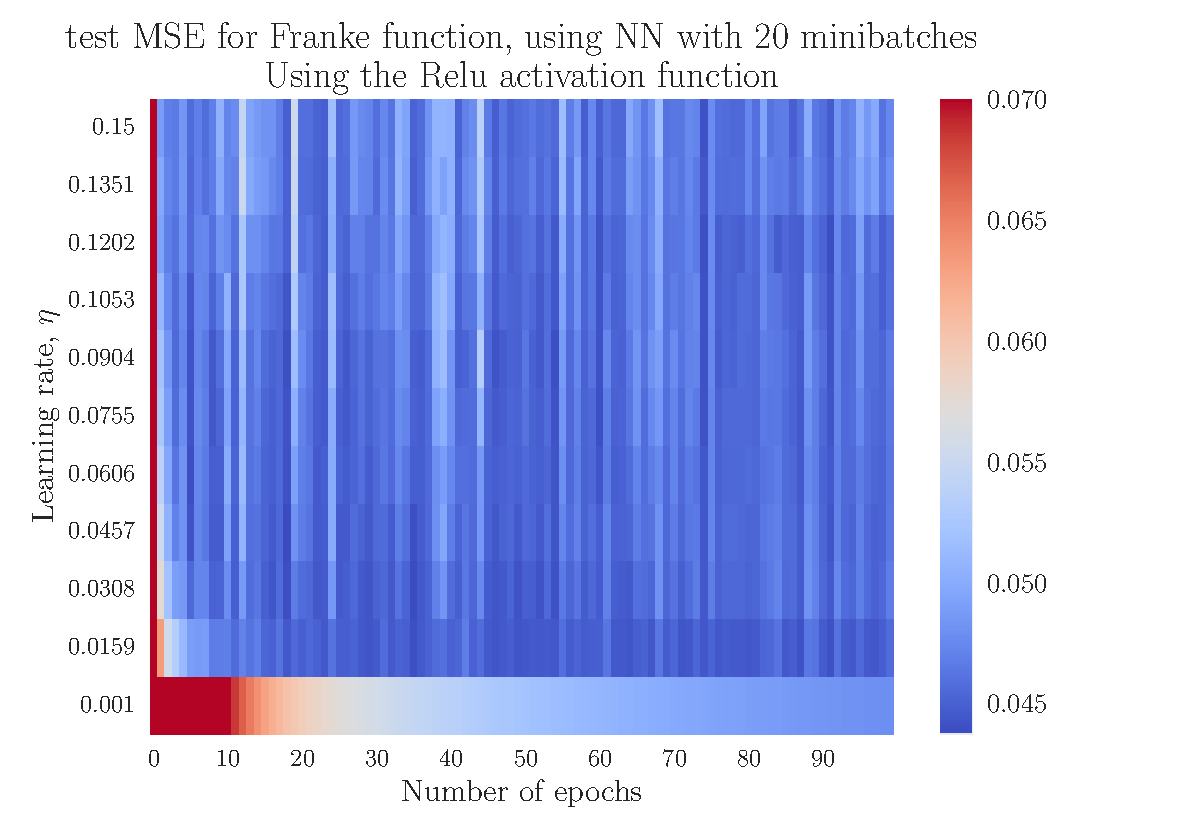
\includegraphics[width=\linewidth]{../output/plots/NN_Franke__epochs_eta__test_MSE__relu__705262.pdf}
	\endminipage\hfill
	\minipage{0.49\textwidth}
	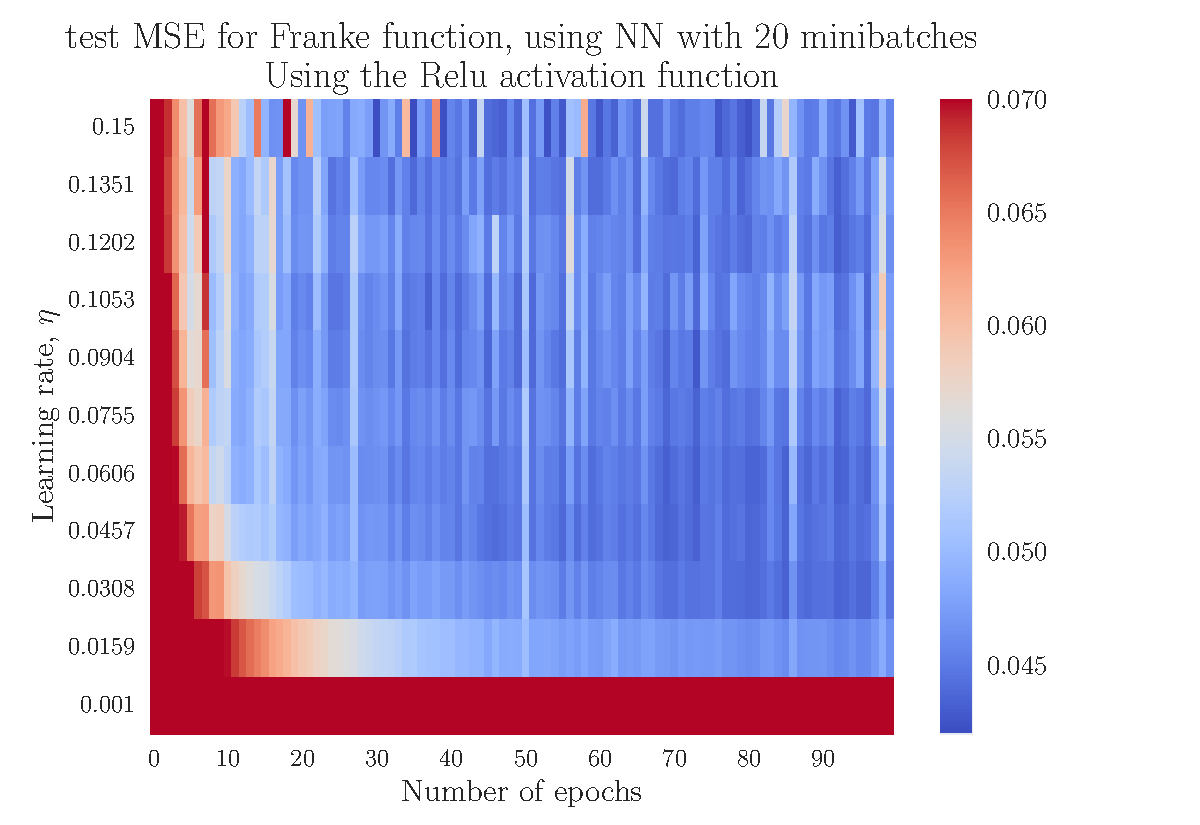
\includegraphics[width=\linewidth]{../output/plots/NN_Franke__epochs_eta__test_MSE__relu__45014.pdf}
	\endminipage\hfill
	\minipage{0.49\textwidth}
	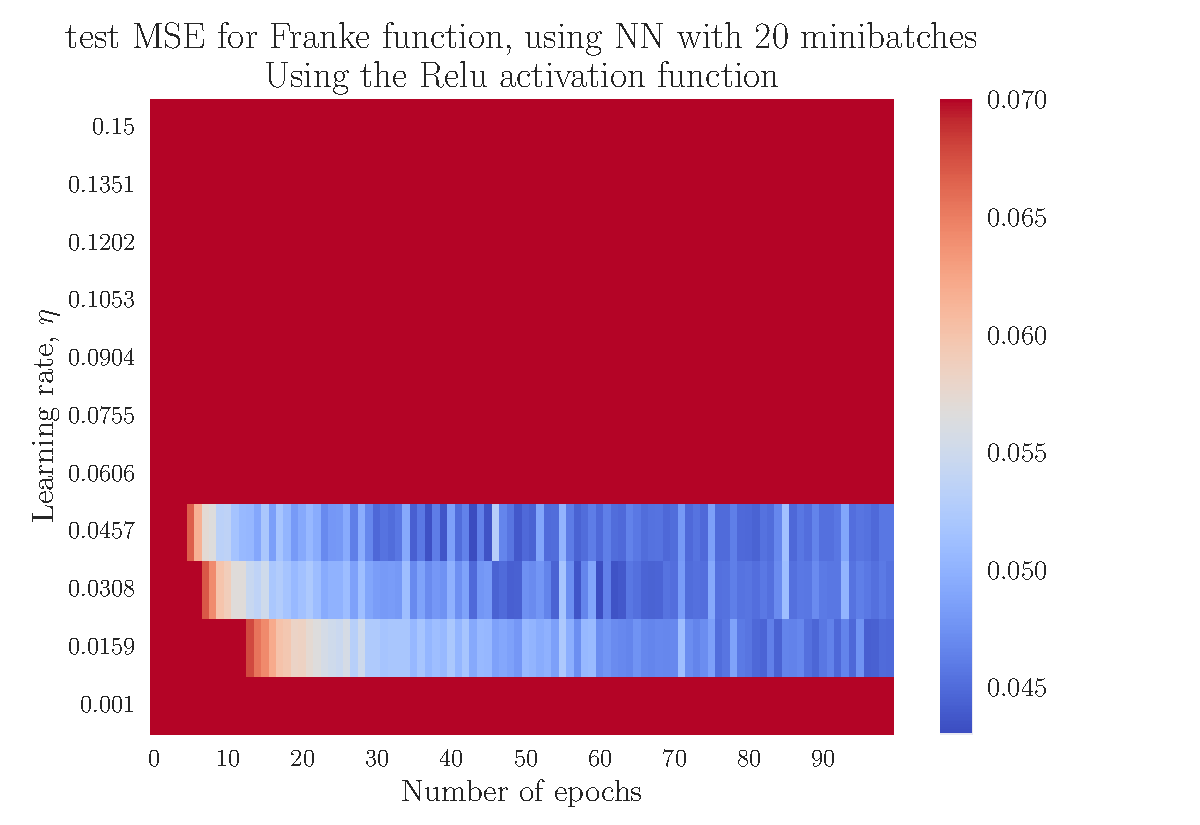
\includegraphics[width=\linewidth]{../output/plots/NN_Franke__epochs_eta__test_MSE__relu__704482.pdf}
	\endminipage
	\caption{Neural networks with different number of layers, but same number of total nodes. Top left has 1 hidden layer, top right has 2. Bottom left has 3, while bottom right has 4. All have a total of 20 nodes.}\label{fig:NN_class_layers}
\end{figure}


\subsubsection{Logistic Regression}

In figure \ref{fig:logreg_eta_epoch} we plot the accuracy score as a function of epochs, for different learning rates $\eta$ and $L_2$ parameter set to $\lambda = 0$. The top plot is for the train data, and bottom for test data. As mentioned we want to see how the network learns, meaning that we are not that interested in the precise accuracy score before we perform a grid search. First, looking at the train accuracy, when $\eta \leq 3\cdot 10^{-5}$ we do not converge within the 200 epochs. We also notice unstable accuracy for $\eta\geq 0.1122$. These effects is more apparent in the test accuracy, where we see clear variations in accuracy at $\eta \geq 0.03981$, and non converging accuracy at $\eta\leq 8\cdot 10^{-5}$. The optimal learning rate should therefore be within $8\cdot 10^{-5} \geq \eta \leq 0.1122$.

\begin{figure}[h]
	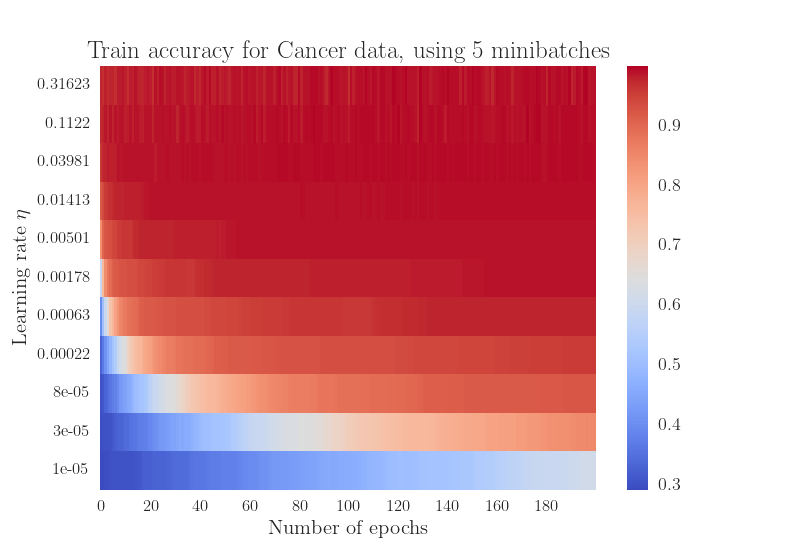
\includegraphics[width=\linewidth]{../output/plots/reg_Cancer__epochs_eta__Train_accuracy__705107.png}
	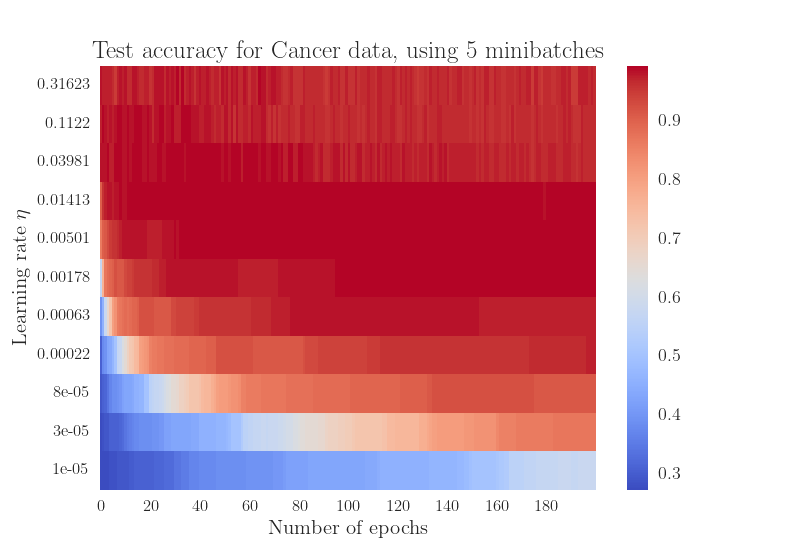
\includegraphics[width=\linewidth]{../output/plots/reg_Cancer__epochs_eta__Test_accuracy__924831.png}
	\caption{These two figures illustrates how the accuracy score evolves as a function of epochs ($x$-axis) and learning rate $\eta$ ($y$-axis) (for logistic regression). An accuracy score of one corresponds to 100\% correct classifications.}\label{fig:logreg_eta_epoch}
\end{figure}

In figure \ref{fig:logreg_eta_lambda} we have plotted the results from our grid search. There we have displayed the precise test accuracy score, as a function of learning rate $\eta$ and hyper parameter $\lambda$. Looking at the figure, we notice that our best accuracy score is 99.1\%, for $0.001 \geq \eta \leq 0.00631$ and all $\lambda$'s. We acquire the same accuracy score for $\eta = 0.01585$ and $\lambda\geq 10^{-3.6}$. This is the exact same accuracy as when using Scikit-Learn's logistic regression with $L_2$ regularization, and corresponds to one miss-categorization.

\begin{figure}[h]
	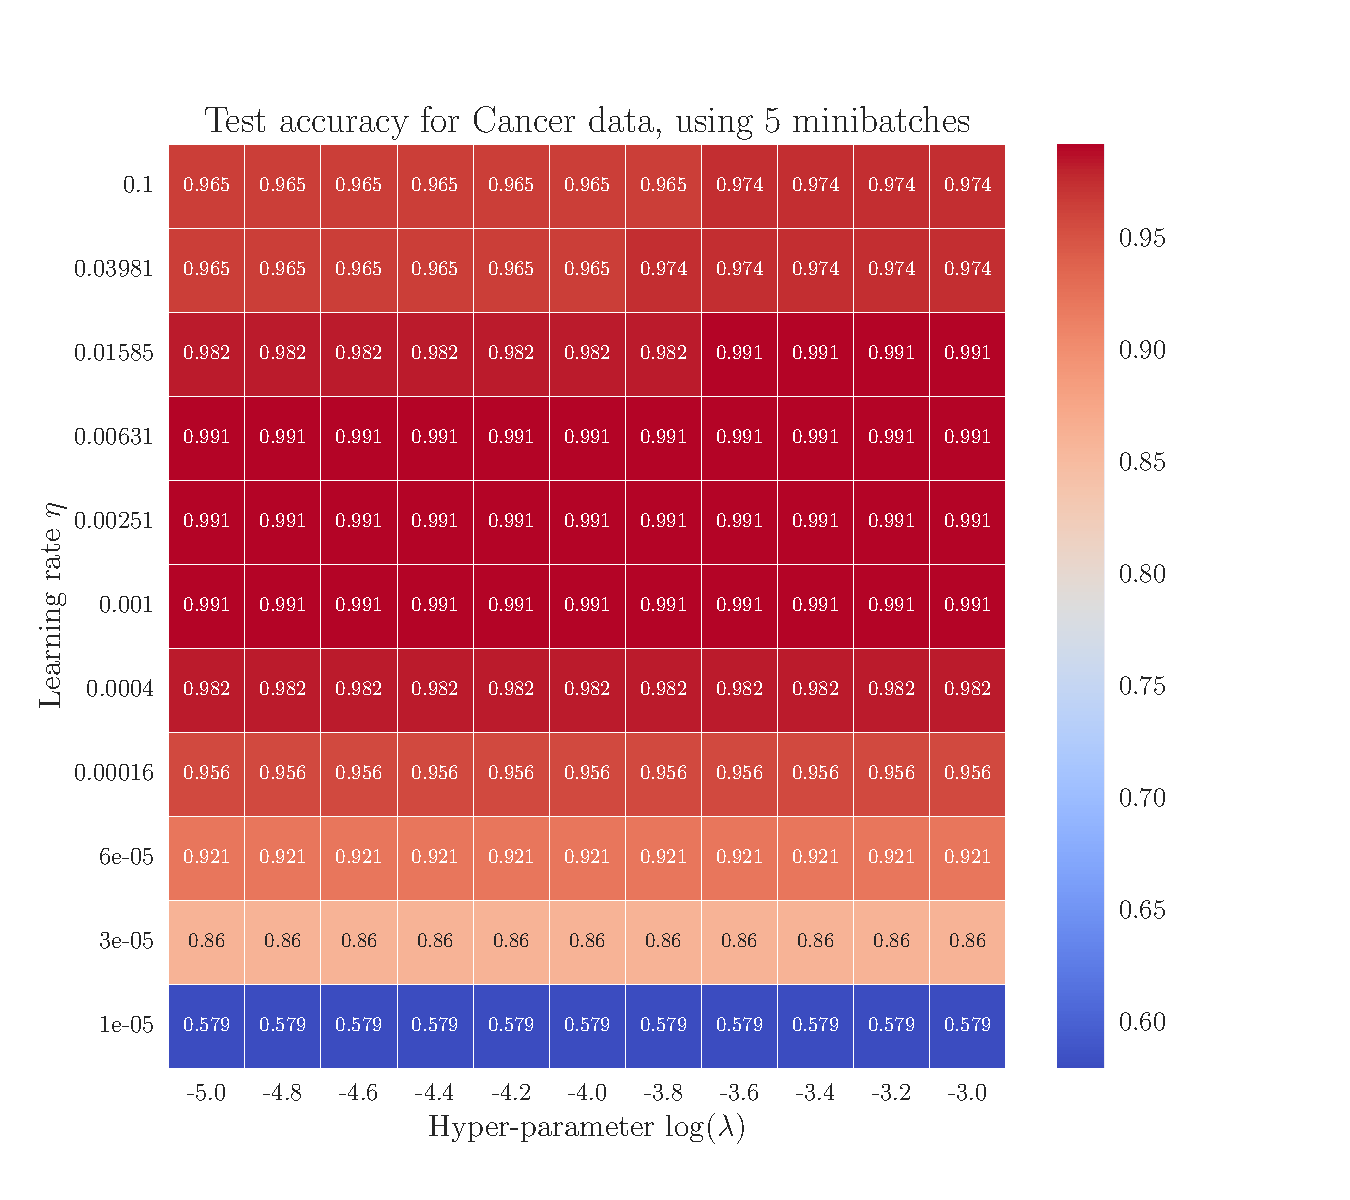
\includegraphics[width=\linewidth]{../output/plots/reg_Cancer__lambda_eta__Test_accuracy__860729.pdf}
	\caption{Here we have plotted the accuracy for the test data, as a function of both learning rate $\eta$ ($y$-axis) and logarithm of hyper parameter $\lambda$ ($x$-axis) (for logistic regression). An accuracy score of one corresponds to 100\% correct classification.}\label{fig:logreg_eta_lambda}
\end{figure}

There are many potential optimal parameters, however lets choose $\eta= 0.00251$ and $\lambda = 0$, and print the number of cases where our output is withing (0.1, 0.9). We remind that this is not a very comprehensive analysis, and we talk more about this in the discussion-section. Nevertheless, after the first epoch we have 58 cases, and after 200 epochs we have eight cases where the output is within (0.1, 0.9).

\clearpage

\section{Discussion}

We know that the optimal value for a given parameter might not be the same, when we change values of other parameters. Meaning that this method is then not guaranteed to optimize the entire parameter space. However, we can assume it will be a good approximation, and will save a great deal of time.

We could have chosen other shapes for the dynamic learning rate, for instance exponential decreasing $\eta$, or an upside-down sigmoid. It can be useful to study the effects of different learning schedules, though this is outside the scope of this paper.

would have been nice to plot eta vs momentum, to see where they work well together. but momentum is used to get fast convergence, so we only did momentum epochs.

FF NEURAL NETWORK FRANKE:




The fact that we obtain the same accuracy (99.2\%) as when using Scikit-Learn's logistic regression, gives us confidence in our results. The 99.2\% accuracy corresponds to one miss-classification. We do not believe it feasible to better this result, given that a professionally written library yields the same. One area which we would have liked to analyze further is the confidence of our algorithm. After 200 epochs, for $\eta = 0.00251$ and $\lambda = 0$, we had eight cases where the output was within (0.1, 0.9). That threshold is arbitrary, however it illustrates potential further analysis. To find the optimal parameters we should not only analyze accuracy, but also minimize the number of cases which one deems to inconclusive. Methods of optimization one could try, is implementing different output functions, initialization of weights and bias and momentum parameter \eqref{eq:vt_mom}.

\section{Conclusion}


\bibliographystyle{plain}
\bibliography{refs}
\end{document}

